\documentclass[14pt, a4paper]{extarticle}
\usepackage{amsmath}
\usepackage{graphicx}
\usepackage[table,xcdraw]{xcolor}
\usepackage{matlab-prettifier}
\usepackage[margin=1in]{geometry}
\usepackage{calc}
\usepackage{eso-pic}
\usepackage{pgfplots}
\usepackage{tikz}
\usepackage{multirow}
\usepackage{longtable}
\usetikzlibrary{fillbetween}

\usepackage[bookmarks,hypertexnames=false,debug,linktocpage=true,hidelinks]{hyperref}
\hypersetup{
    colorlinks,
    linktoc=all,
    linkcolor={blue},
    citecolor={blue},
    urlcolor={blue}
}

\usepackage{xepersian}
\settextfont[Scale = 1]{B Nazanin}
% \linespread{3}

% Border
\newlength{\PageFrameTopMargin}
\newlength{\PageFrameBottomMargin}
\newlength{\PageFrameLeftMargin}
\newlength{\PageFrameRightMargin}

\setlength{\PageFrameTopMargin}{1cm}
\setlength{\PageFrameBottomMargin}{1cm}
\setlength{\PageFrameLeftMargin}{1cm}
\setlength{\PageFrameRightMargin}{1cm}

\makeatletter

\newlength{\Page@FrameHeight}
\newlength{\Page@FrameWidth}

\AddToShipoutPicture{
  \thinlines
  \setlength{\Page@FrameHeight}{\paperheight-\PageFrameTopMargin-\PageFrameBottomMargin}
  \setlength{\Page@FrameWidth}{\paperwidth-\PageFrameLeftMargin-\PageFrameRightMargin}
  \put(\strip@pt\PageFrameLeftMargin,\strip@pt\PageFrameTopMargin){
    \framebox(\strip@pt\Page@FrameWidth, \strip@pt\Page@FrameHeight){}}}

\makeatother

% Border

\begin{document}

\newpage
	\begin{titlepage}
	\centering
	\begin{figure}
		\centering
		
\includegraphics[scale = 0.4]{kn-toosi.png}
	\end{figure}
	% Course Title
	{\Huge \textbf{کنترل مبتنی بر پیش‌بینی مدل}}
	\par
	\vspace{0.5cm}
	
	% Teacher's Name
	{\large دکتر امیرحسین نیکوفرد}\par\vspace{1cm}
		\vspace{1cm}
	
	{\LARGE تمرین سری سوم}
	\par
	\vspace{3cm}
	
	% Student Name
	{\LARGE \textbf{سید محمد امین غضنفری}}
	\par
	\vspace{1cm}
	
	\textbf{شماره دانشجویی:}
	{\large 40209104}
	\vspace{4cm}
	
	% Year
	{\Large پاییز 1403}

	\end{titlepage}

\newpage

\tableofcontents

\newpage

\section{سوال اول}
\subsection{بخش اول}

تابع تبدیل به صورت زیر در اختیار قرار دارد:\\
\[
G(s) = \frac{F(s)}{U(s)} = \frac{k_{sp} K_s k_e (A_i + A_0)}{(\tau s + 1) \left[ (K_p + Cs)(m_a s^2 + d s + k_e) + (A_i^2 s + A_0^2 s) \right]}
\]
با توجه به روش تحقق مینیمال داریم:
\[
G(s) = \frac{Y(s)}{U(s)} = \frac{\beta}{s^n + \alpha_1 s^{n-1} + \dots + \alpha_{n-1}s + \alpha_n}
\]

\[
\dot{x}(t) = 
\begin{bmatrix}
	0 & 1 & 0 & \dots & 0 \\
	0 & 0 & 1 & \dots & 0 \\
	\vdots & \vdots & \vdots & \ddots & \vdots \\
	0 & 0 & 0 & \dots & 1 \\
	-\alpha_n & -\alpha_{n-1} & -\alpha_{n-2} & \dots & -\alpha_1
\end{bmatrix}
x(t)
+
\begin{bmatrix}
	0 \\
	0 \\
	\vdots \\
	0 \\
	\beta
\end{bmatrix}
u(t)
\]
\[
y(t) = 
\begin{bmatrix}
	1 & 0 & 0 & \dots & 0
\end{bmatrix}
x(t)
\]

مقادیر مربوطه به شرح زیر به دست می‌آیند.
\[
\begin{aligned}
	\left\{
	\begin{aligned}
		\alpha_1 &= \frac{\left( \tau (K_p m_a + C d) + C m_a \right)}{\tau C m_a} \\
		\alpha_2 &= \frac{\left( \tau (K_p d + C k_e + A_i^2 + A_0^2) + (K_p m_a + C d) \right)}{\tau C m_a} \\
		\alpha_3 &= \frac{\left( \tau K_p k_e + (K_p d + C k_e + A_i^2 + A_0^2) \right)}{\tau C m_a} \\
		\alpha_4 &= \frac{K_p k_e}{\tau C m_a} \\
		\beta &= \frac{k_{sp} K_s k_e (A_i + A_0)}{\tau C m_a}
	\end{aligned} \right. 
\end{aligned}
\]

%\[
%G(s) = \frac{F(s)}{U(s)} = \frac{k_{sp} k_e k_p (A_i + A_0)}{
%	\tau C m_a s^4 + \left( \tau (K_p m_a + C d) + C m_a \right) s^3 + \left( \tau (K_p d + C k_e + A_i^2 + A_0^2) + (K_p m_a + C d) \right) s^2 + \left( \tau K_p k_e + (K_p d + C k_e + A_i^2 + A_0^2) \right) s + K_p k_e
%}
%\]

حال با استفاده از آن‌ها، معادلات فضای حالت را محاسبه و ماتریس‌های آن را به دست می‌آوریم.\\
\[
A = 
\begin{bmatrix}
	0 & 1 & 0 &  0 \\
	0 & 0 & 1 &  0 \\
	0 & 0 & 0 &  1 \\
	-\alpha_4 & -\alpha_3 & -\alpha_2 & -\alpha_1
\end{bmatrix}, 
B = \begin{bmatrix}
	0 \\
	0 \\
	0 \\
	\beta
\end{bmatrix}, 
C = \begin{bmatrix}
	1 & 0 & 0 & 0
\end{bmatrix}, D = 0
\]
\newpage
\subsection{بخش دوم}
برای این بخش ابتدا باید نایقینی‌ها را به نحوی به سیستم اعمال کنیم. برای این منظور، از خاصیت تابع سینوس که مقداری بین 0 و 1 دارد استفاده می‌کنیم. به عنوان مثال برای 
$k_e$
محاسبات مربوطه را انجام می‌دهیم. برای بقیه پارامترها نیز محاسبات به همین صورت خواهد بود.\\
\[
k_e = (100 + 50)/2 + [(100 - 50)/2] \times sin(t) = 75 + 25 sin(t)
\]
برای سایر مقادیر داریم:\\
\[
\begin{aligned}
K_s &= 0.375 + 0.125 * sin(t)\\           
K_p &= 2.5 \times 10^{-12} + 2.5 \times 10^{-12} * sin(t)\\       
C &= 2 \times 10^{-11} + 10^{-11} * sin(t)\\            
d &= 700 + 100 * sin(t)\\              
m_a &= 20.0 + 0.1 * sin(t)\\             
A_i &= 0.00203 + 0.0001 * sin(t)\\       
A_o &= 0.00152 + 0.00008 * sin(t)\\      
k_{sp} &= 0.0012 + 0.0001 * sin(t)\\      
\tau &= 35 + 5 * sin(t);  
\end{aligned}
\]

حال در سیمولینک سیستم را طراحی می‌کنیم.\\
\begin{figure}[h!]
	\centering
	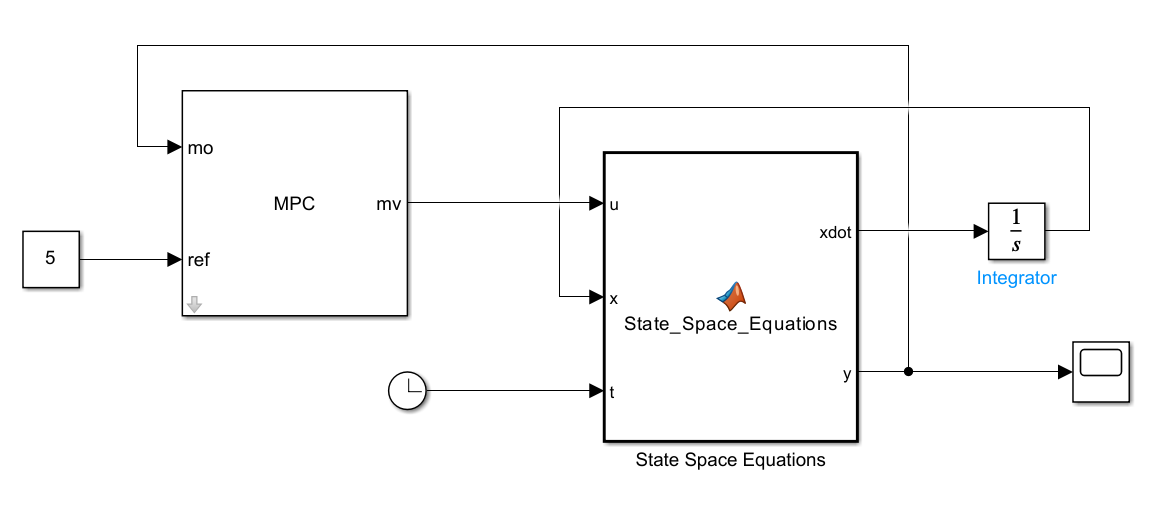
\includegraphics[scale = 0.6]{Q1_2_sim.png}
	\caption{سیستم با کنترلر 
	\lr{linear MPC}}
\end{figure}
\newpage
معادلات قرار گرفته در 
\lr{Matlab Function}
در ادامه آورده شده است.\\
\begin{latin}
	\begin{lstlisting}[frame=single,numbers=left,style=Matlab-Pyglike]
function [xdot, y] = State_Space_Equations(u, x, t)

% Parameter ranges pertaining to the linear transfer function (Table 1)

ke = 75 + 25 * sin(t);
Ks = 0.375 + 0.125 * sin(t);
Kp = 2.5*10^(-12) + 2.5*10^(-12) * sin(t);
C1 = 2*10^(-11) + 1*10^(-11) * sin(t);
d = 700 + 100 * sin(t);
ma = 20.0 + 0.1 * sin(t);
Ai = 0.00203 + 0.0001 * sin(t);
Ao = 0.00152 + 0.00008 * sin(t);
ksp = 0.0012 + 0.0001 * sin(t);
tau = 35 + 5 * sin(t);      

% Definig the parameters calculated for the state-space equations

a1 = (tau * (Kp * ma + C1 * d) + (C1 * ma)) / (tau * C1 * ma);
a2 = (tau * (Kp * d + C1 * ke + Ai^2 + Ao^2) + (Kp * ma + C1 * d)) / (tau * C1 * ma);
a3 = (tau * Kp * ke + Kp * d + C1 * ke + Ai^2 + Ao^2) / (tau * C1 * ma);
a4 = (Kp * ke) / (tau * C1 * ma);
beta = (ksp * Ks * ke * (Ai + Ao)) / (tau * C1 * ma);

% State-Space Matrices

A = [
0,1,0,0;
0,0,1,0;
0,0,0,1;
-a4,-a3,-a2,-a1
];

B = [
0;
0;
0;
beta
];

C = [1,0,0,0]; 

% State-Space equations

xdot = A * x + B * u;
y = C * x;
	\end{lstlisting}
\end{latin}

همچنین مقادیر مربوط به کنترلر در تصویر زیر قابل مشاهده است.\\

\begin{figure}[h!]
	\centering
	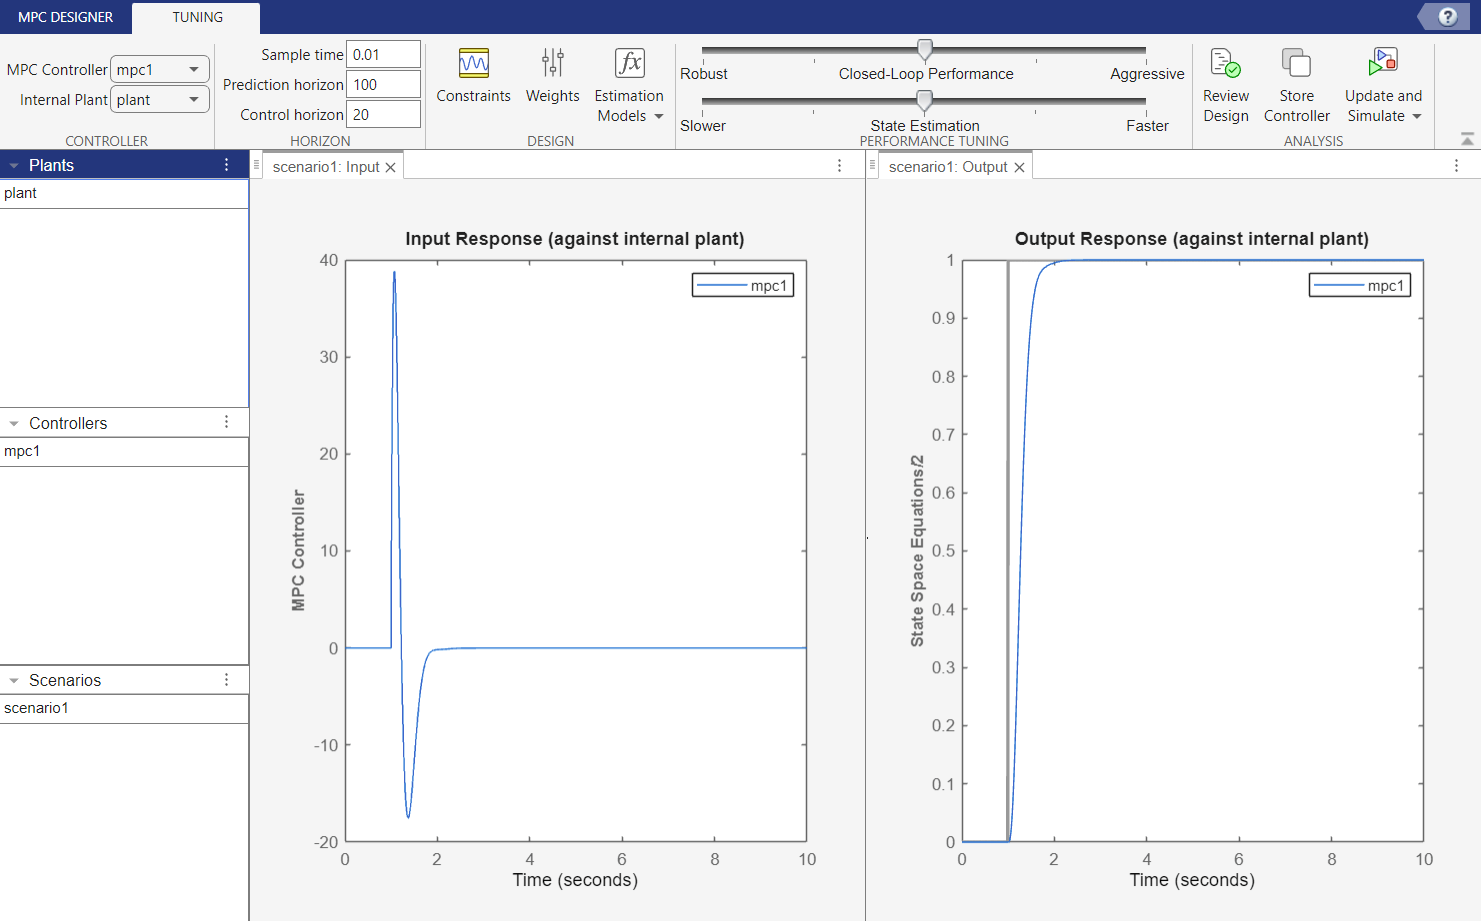
\includegraphics[scale = 0.5]{Q1_2_mpc.png}
	\caption{صفحه مربوط به 
		\lr{linear MPC}}
\end{figure}
\newpage
در نهایت هم خروجی سیستم به صورت زیر به دست آمده است.
\begin{figure}[h!]
	\centering
	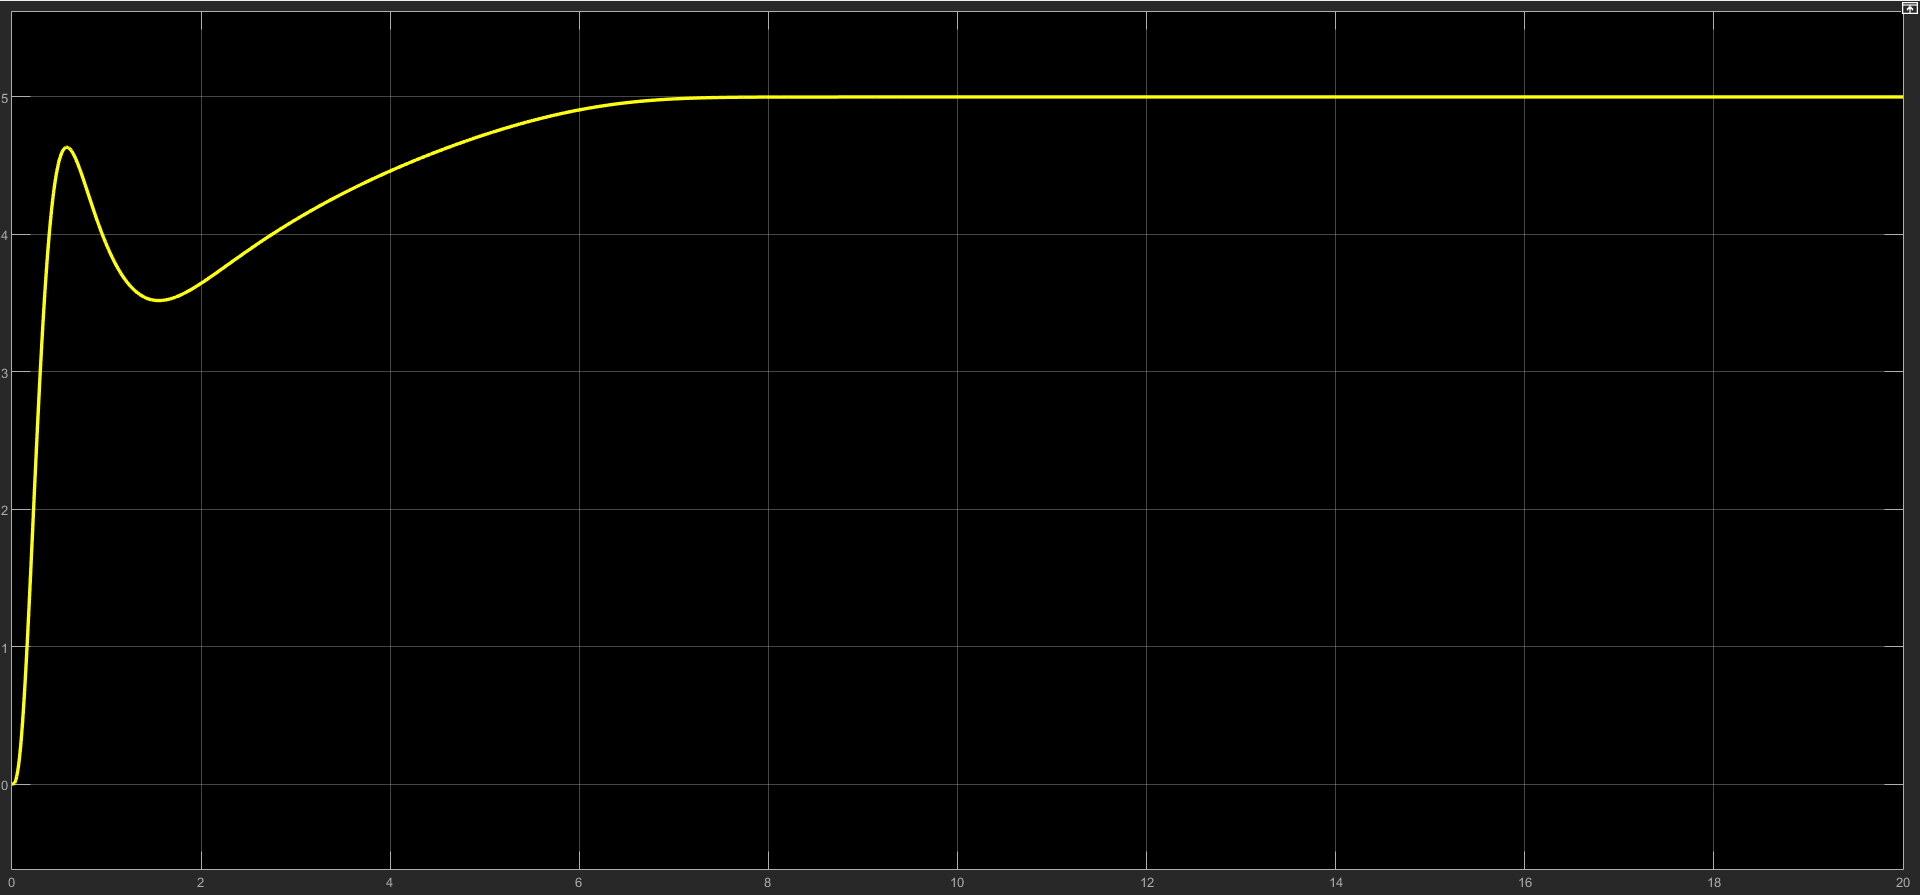
\includegraphics[scale = 0.4]{Q1_2_result.png}
	\caption{خروجی سیستم با کنترلر 
		\lr{linear MPC}}
\end{figure}

همانطور که از تصویر پیداست سیستم توانسته پس از 7 ثانیه به تعادل رسیده و مقدار مطلوب ما را دنبال کند. در ابتدا اما یک فراجهش قبل از رسیدن به مقدار نهایی داشته که این رفتار سیستم می‌تواند به دلیل نایقینی موجود در سیستم باشد.
\newpage
\subsection{بخش سوم}
در این بخش، اغتشاش خواسته شده را به سیستم اعمال می‌کنیم و اثر آن بر سیستم را بررسی می‌کنیم.\\
\begin{figure}[h!]
	\centering
	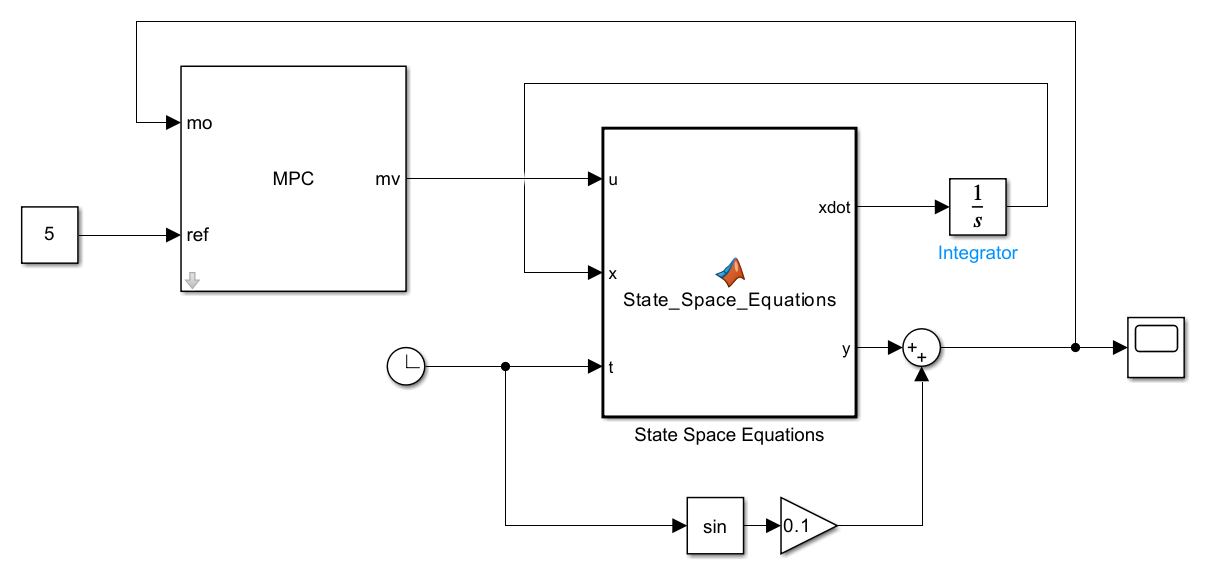
\includegraphics[scale = 0.6]{Q1_3_sim.png}
	\caption{سیستم دارای اغتشاش با کنترلر 
		\lr{linear MPC}}
\end{figure}

با استفاده از همان مقادیر سیستم جدبد را کنترل می‌کنیم.
\begin{figure}[h!]
	\centering
	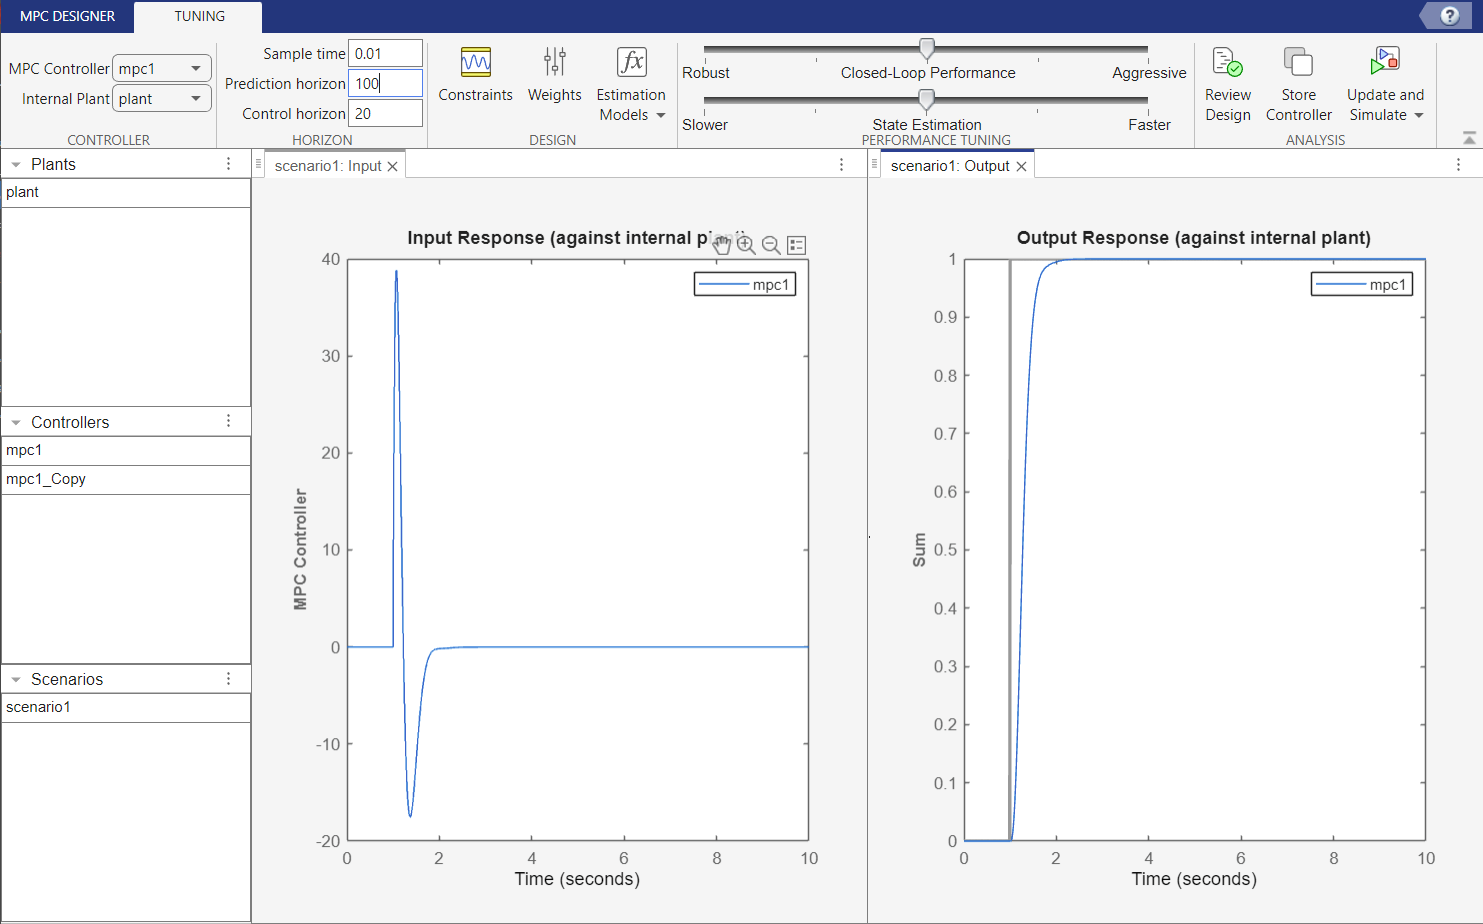
\includegraphics[scale = 0.5]{Q1_3_mpc.png}
	\caption{صفحه مربوط به 
		\lr{linear MPC}}
\end{figure}

\newpage

سیگنال خروجی به صورت زیر به دست می‌آید.
\begin{figure}[h!]
	\centering
	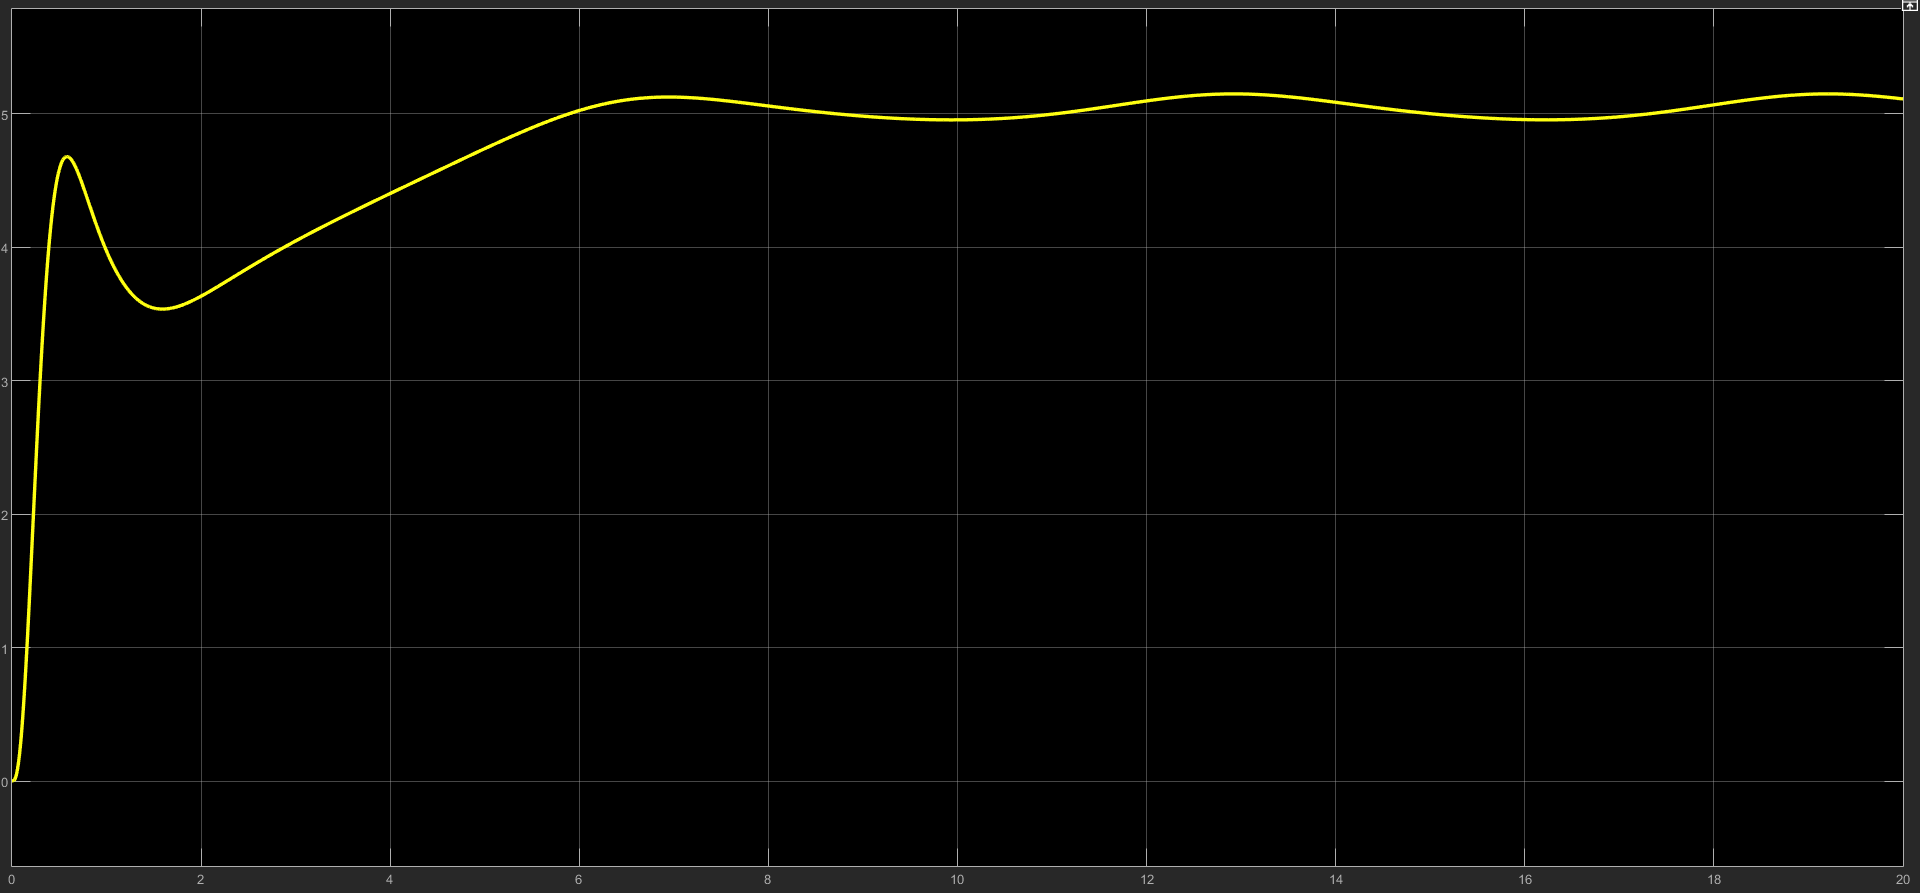
\includegraphics[scale = 0.4]{Q1_3_result.png}
	\caption{خروجی سیستم دارای اغتشاش با کنترلر 
		\lr{linear MPC}}
\end{figure}

سیستم در حال نوسان بین 
$4.95$
و 
$5.15$
است و نمی‌تواند پایدار شود. در واقع کنترلر نمی‌تواند اثر اغتشاش را خنثی کند. همچنین با توجه به بازه نوسان،‌ می‌توان متوجه شد که سیستم دچار خطای ماندگار 
$0.05$
نیز شده است.

\newpage
\subsection{بخش چهارم}

 در بخش سعی می‌کنیم اثرات نایقینی و اغتشاش را با استفاده از کنترلر 
 \lr{tube MPC}
 خنثی کنیم. برای این کار، یک کنترلر 
 \lr{PID}
 به سیستم اضافه کرده و با تعیین پارامتر مناسب برای آن، یه کنترل سیستم می‌پردازیم.
 \begin{figure}[h!]
 	\centering
 	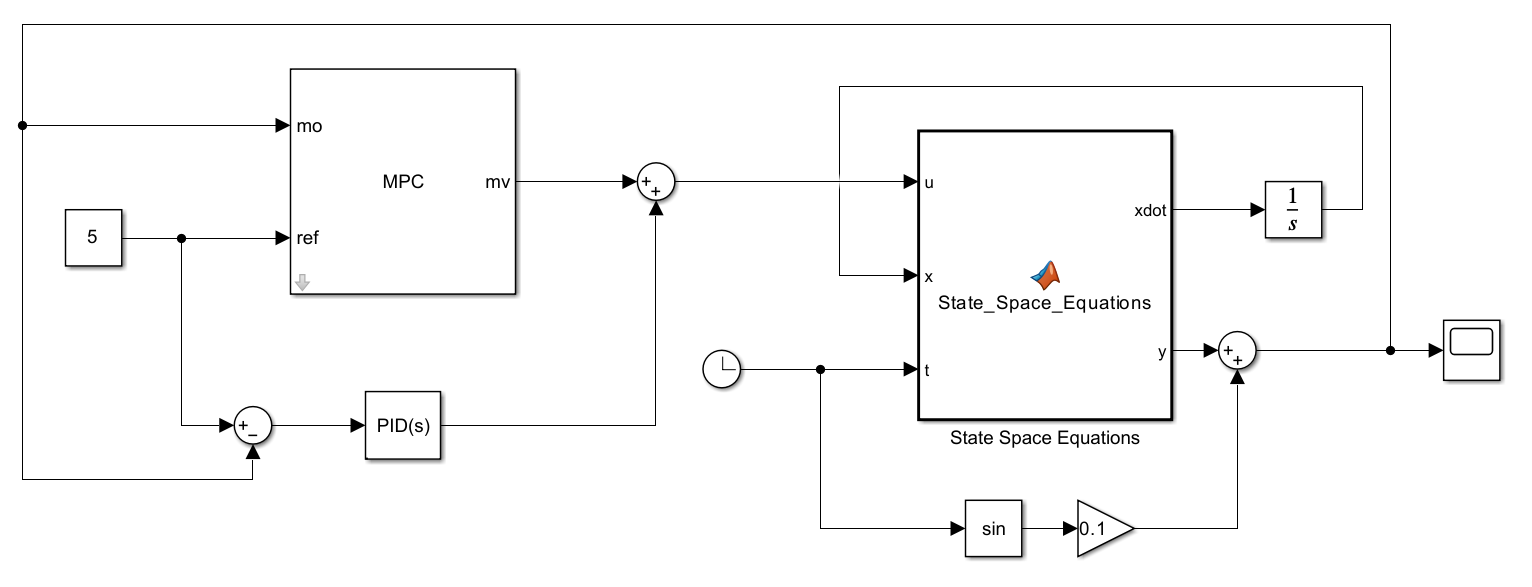
\includegraphics[scale = 0.47]{Q1_4_sim.png}
 	\caption{سیستم دارای اغتشاش با کنترلر 
 		\lr{tube MPC}}
 \end{figure}
 ضرایب 
 \lr{MPC}
 و
 \lr{PID}
 در ادامه قابل مشاهده است.
 \begin{figure}[h!]
 	\centering
 	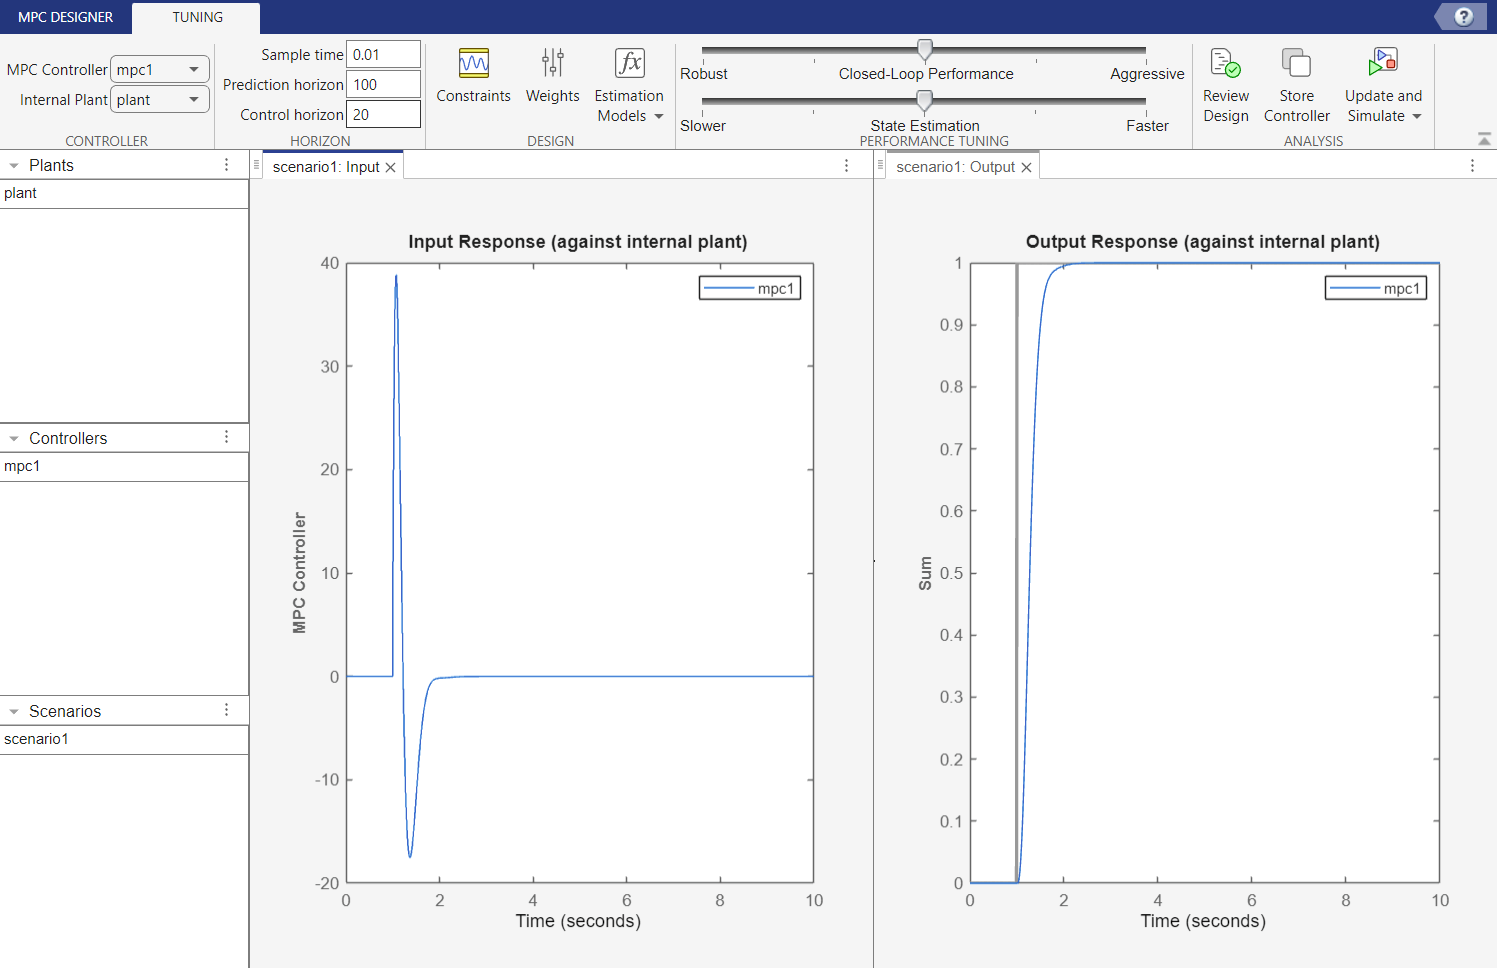
\includegraphics[scale = 0.5]{Q1_4_mpc.png}
 	\caption{صفحه مربوط به 
 		\lr{linear MPC}}
 \end{figure}
 
 \newpage
 
 \begin{figure}[h!]
 	\centering
 	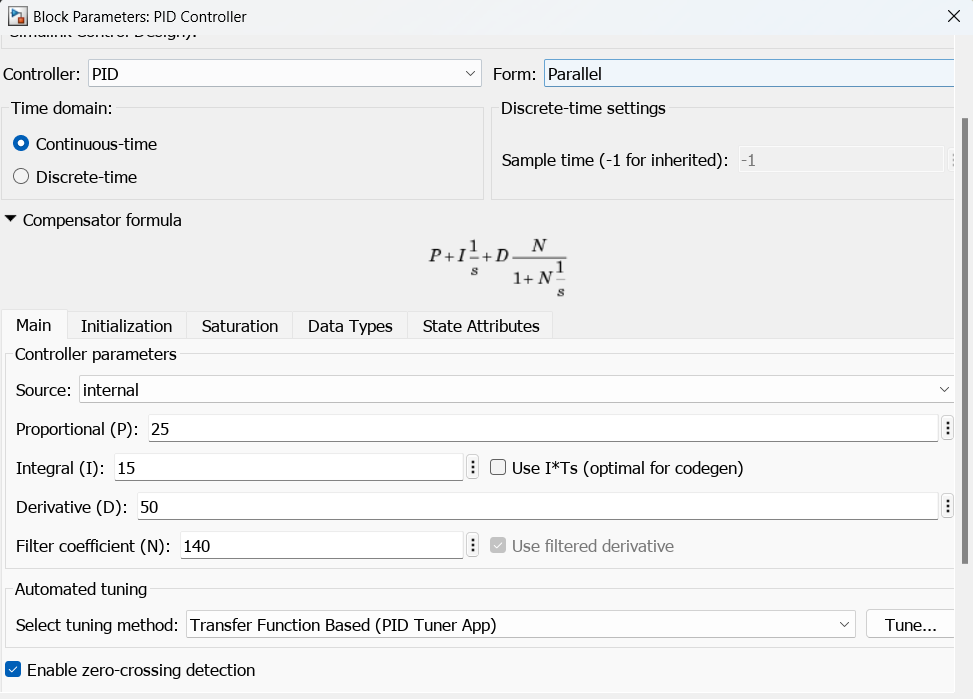
\includegraphics[scale = 0.5]{Q1_4_pid.png}
 	\caption{صفحه مربوط به 
 		\lr{PID}}
 \end{figure}

ضرایب 
\lr{PID}
بعد از استفاده از 
\lr{Auto tune}
مجدد به صورت دستی تنظیم شدند تا نتیجه مطلوب به دست آید. نتیجه این کنترلر در ادامه قابل ملاحظه است.
\begin{figure}[h!]
	\centering
	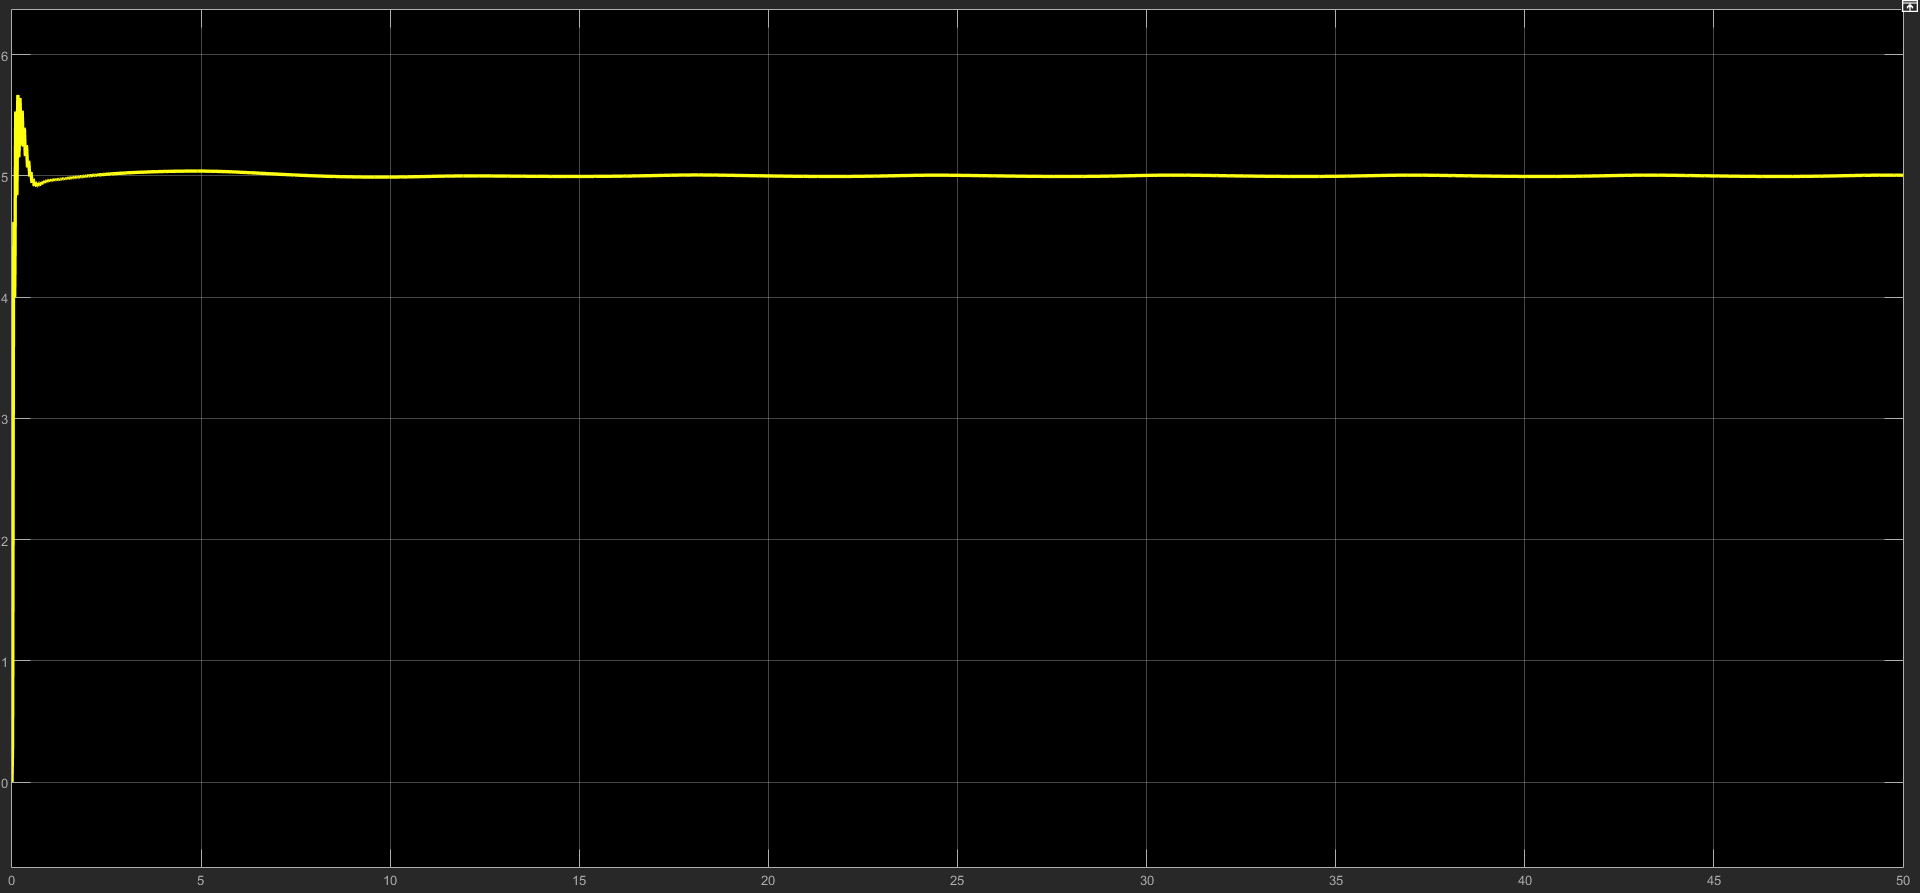
\includegraphics[scale = 0.4]{Q1_4_result1.png}
	\caption{خروجی سیستم دارای اغتشاش با کنترلر 
		\lr{tube MPC}}
\end{figure}


\newpage

تصاویر زیر برای نمایش بهتر خروجی ارائه شده است.

\begin{figure}[h!]
	\centering
	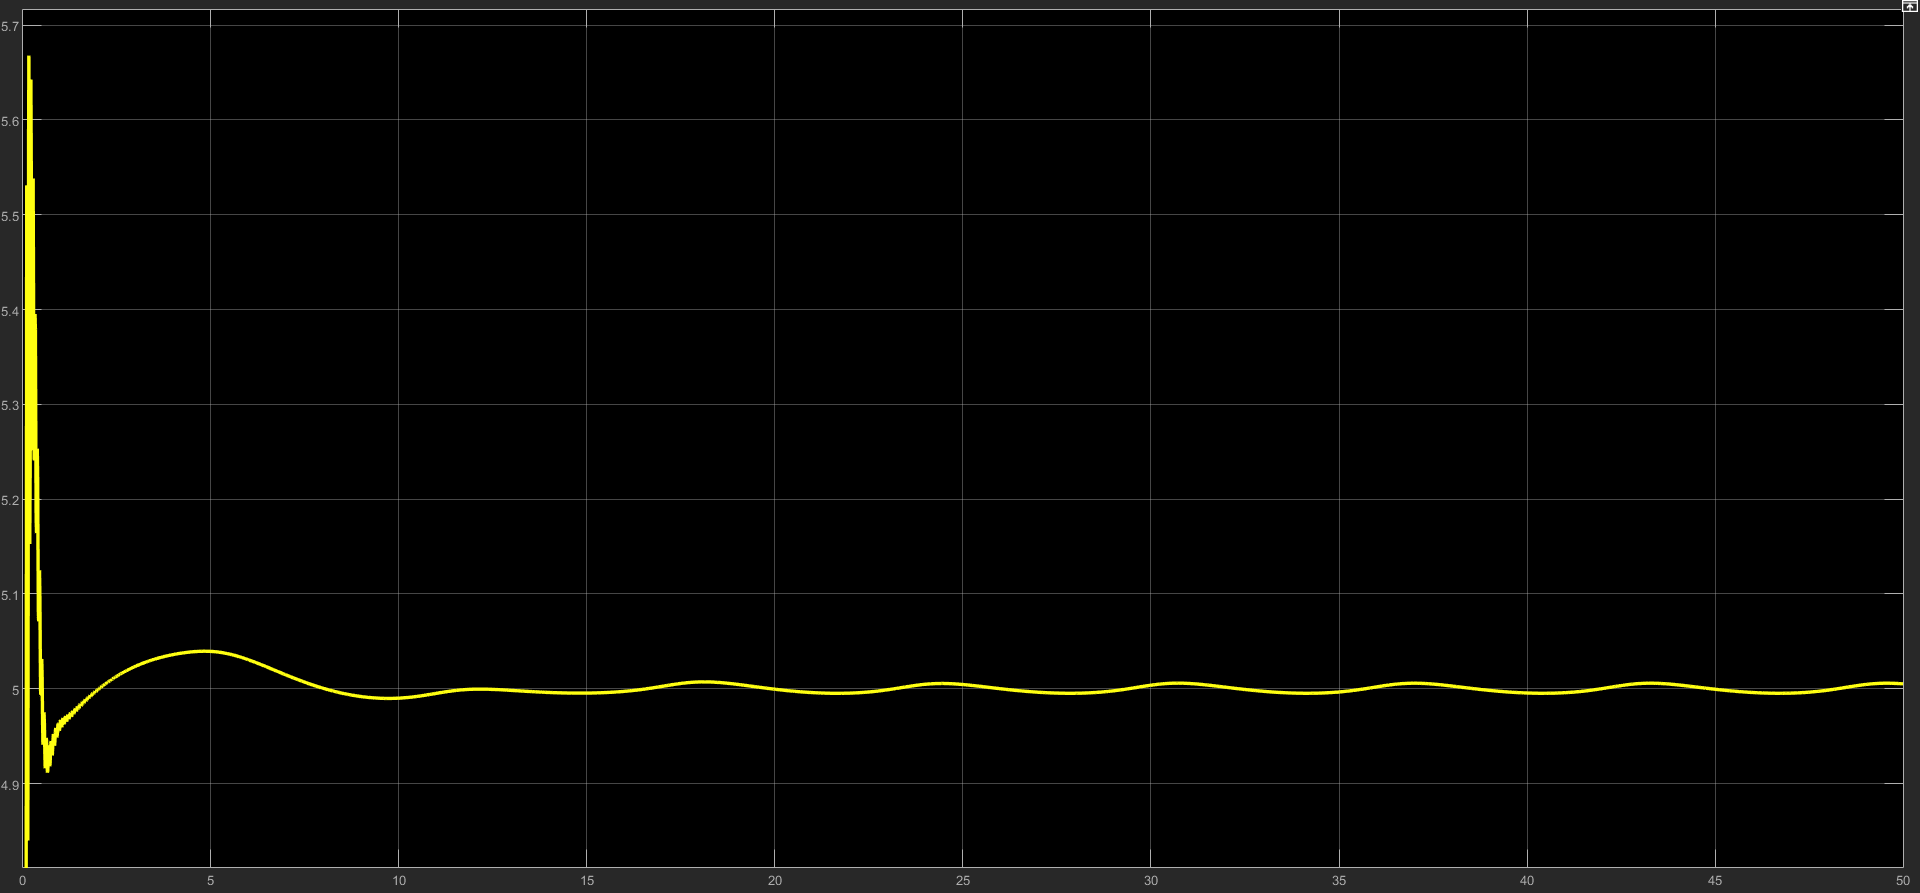
\includegraphics[scale = 0.4]{Q1_4_result2.png}
	\caption{خروجی سیستم دارای اغتشاش با کنترلر 
		\lr{tube MPC}}
\end{figure}

\begin{figure}[h!]
	\centering
	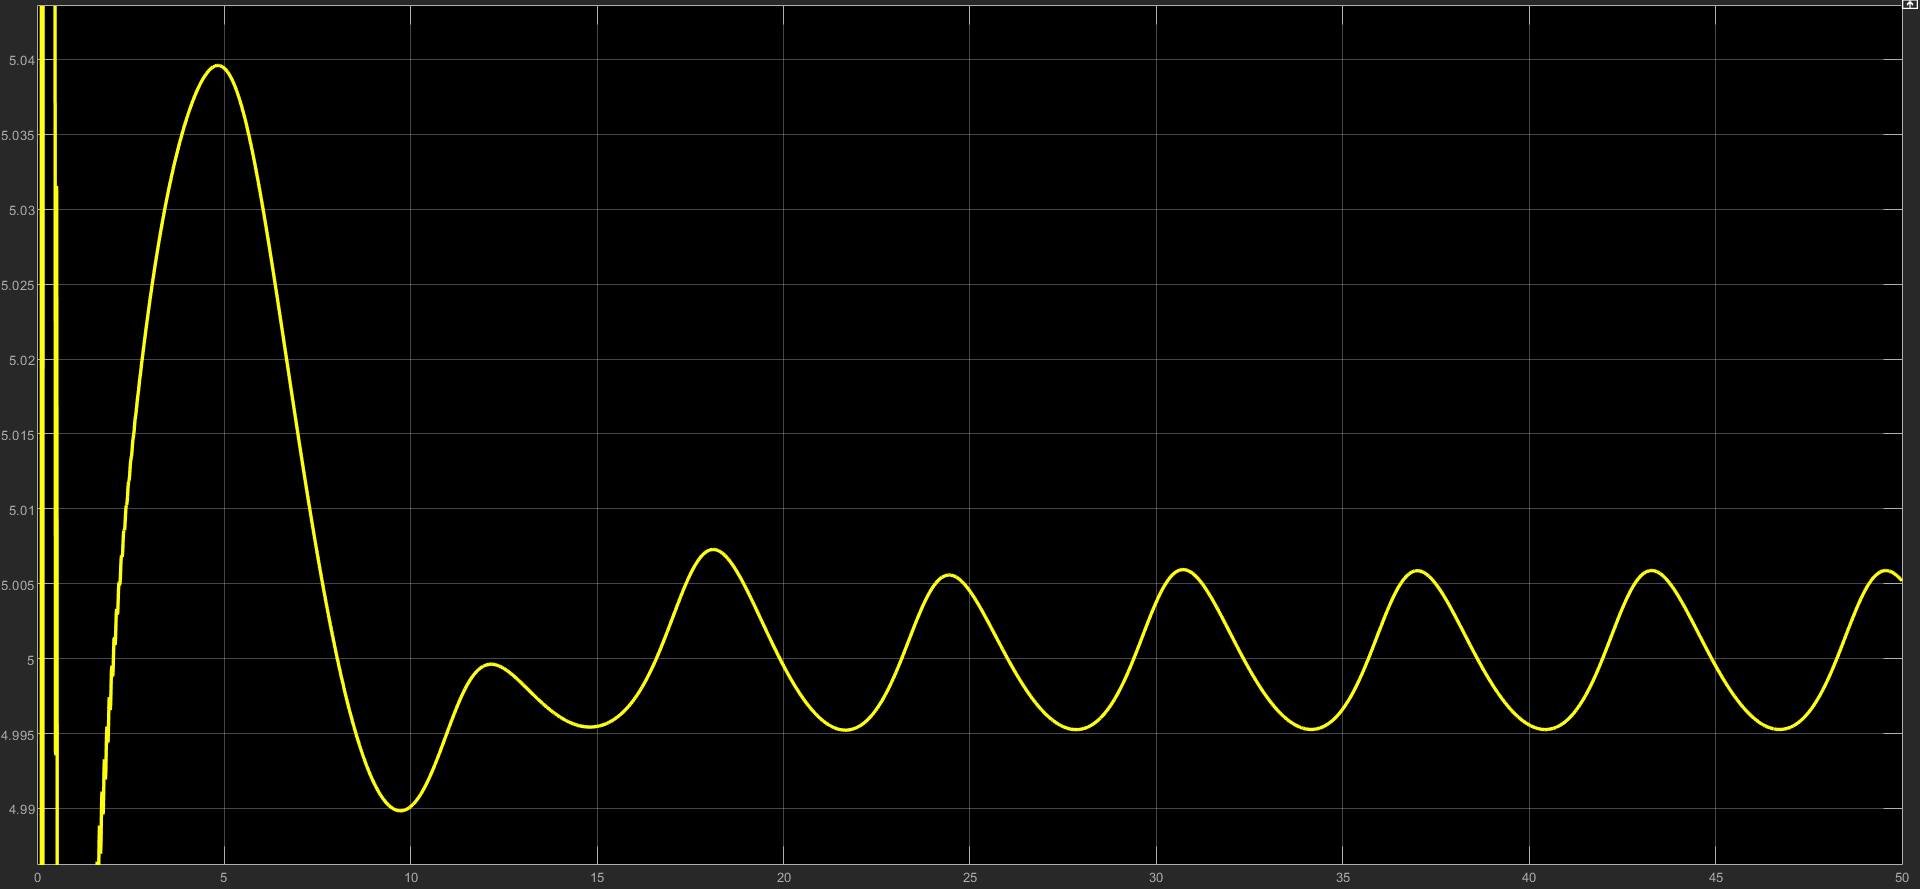
\includegraphics[scale = 0.4]{Q1_4_result3.png}
	\caption{خروجی سیستم دارای اغتشاش با کنترلر 
		\lr{tube MPC}}
\end{figure}

همانطور که مشاهده می‌شود، نوسان سیستم بین 
$4.995$
و 
$5.005$
قرار گرفته و خطای ماندگار آن هم که در قسمت قبل مشاهده کردیم حذف شده است. اما سیستم دچار فراجهشی به بزرگی حدود
$0.65$
شده است. این فراجهش به علت کنترلر 
\lr{PID}
در خروجی سیستم پدید آمده است.
\newpage
\subsection{بخش پنجم}

در این قسمت سعی می‌کنیم با اعمال قید به کنترلر
\lr{mpc}
فراجهش سیستم را کاهش دهیم. قیدی که به سیستم اعمال کردیم،‌مقدار 
$0.1$
بود که کمتر از این مقدار تاثیری روی فراجهش سیستم داشت.

 \begin{figure}[h!]
	\centering
	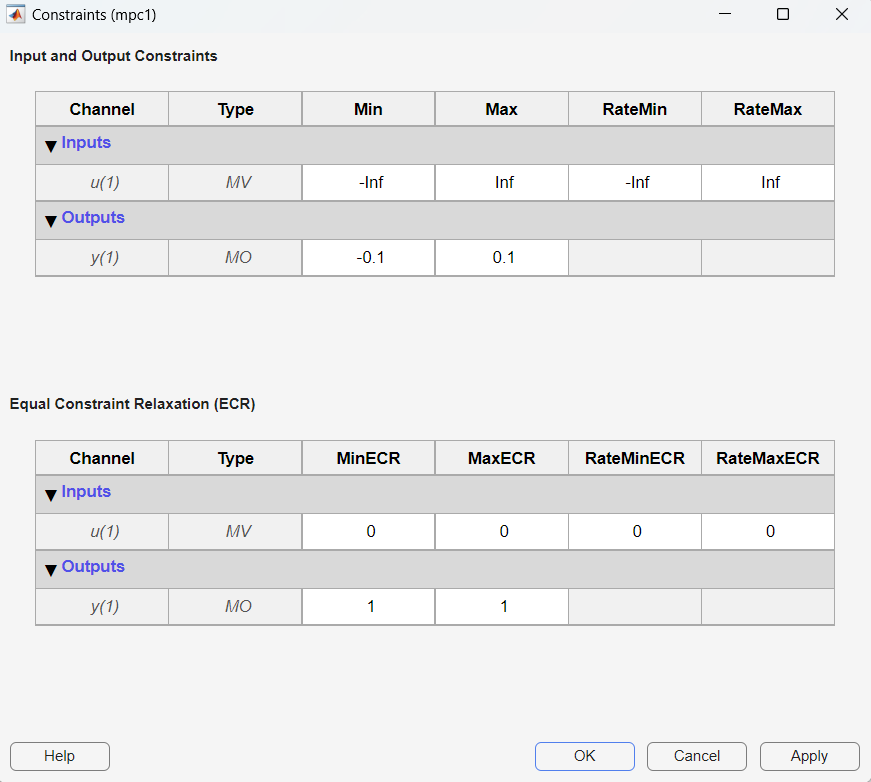
\includegraphics[scale = 0.5]{Q1_5_cons.png}
	\caption{صفحه مربوط به قیود 
		\lr{linear MPC}}
\end{figure}

 \begin{figure}[h!]
	\centering
	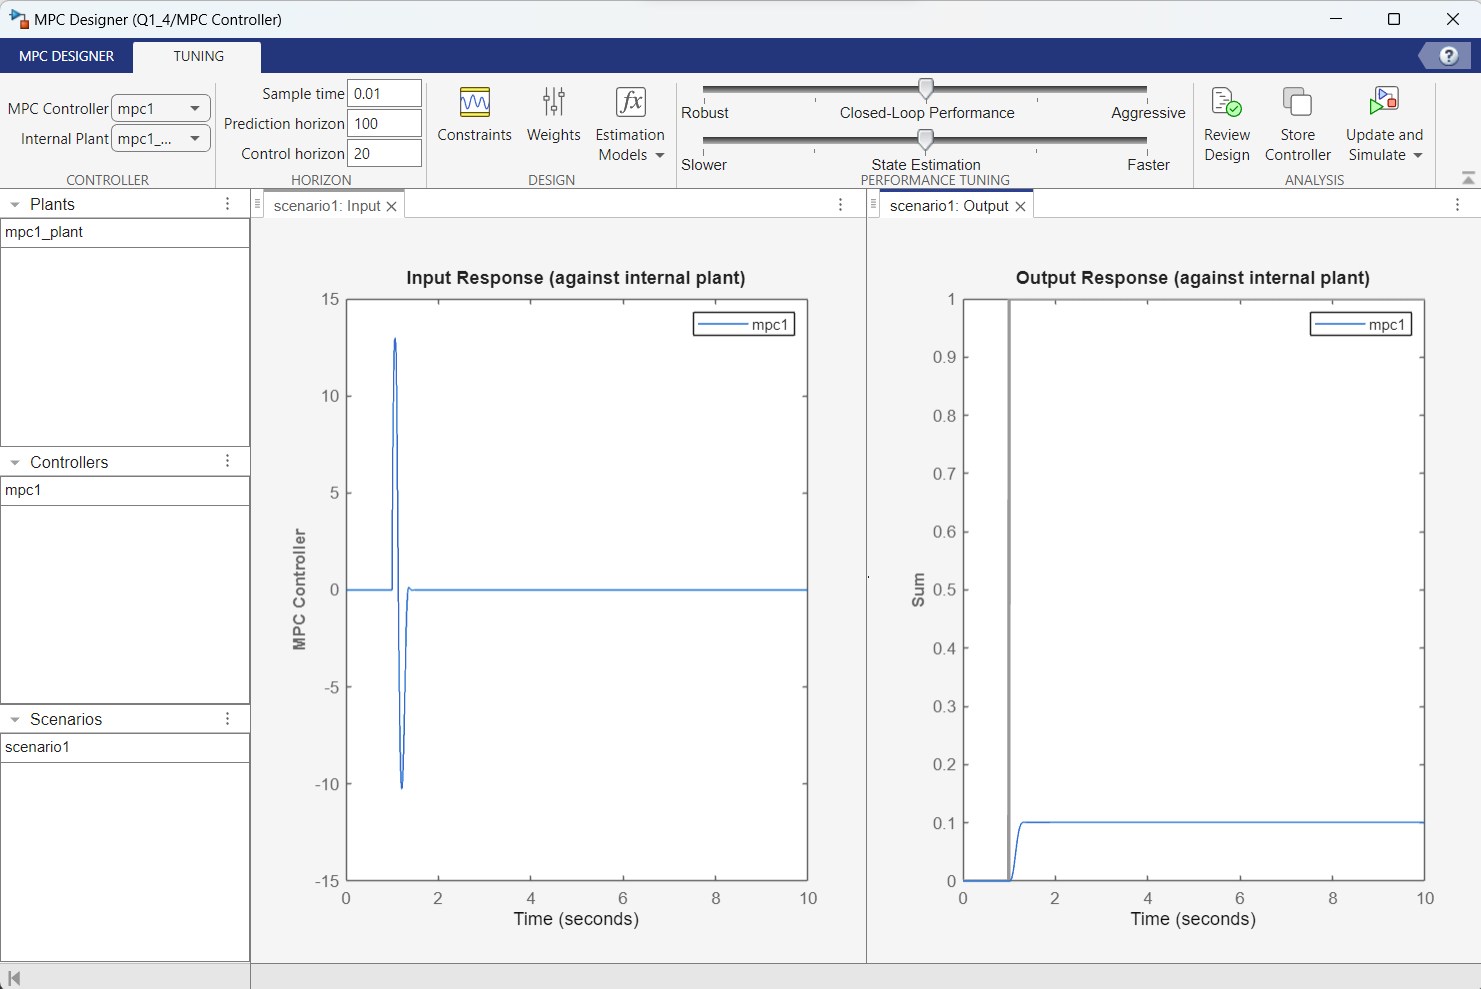
\includegraphics[scale = 0.5]{Q1_5_mpc.png}
	\caption{صفحه مربوط به 
		\lr{linear MPC}}
\end{figure}

نتیجه اعمال این قیود به صورت زیر است.

\begin{figure}[h!]
	\centering
	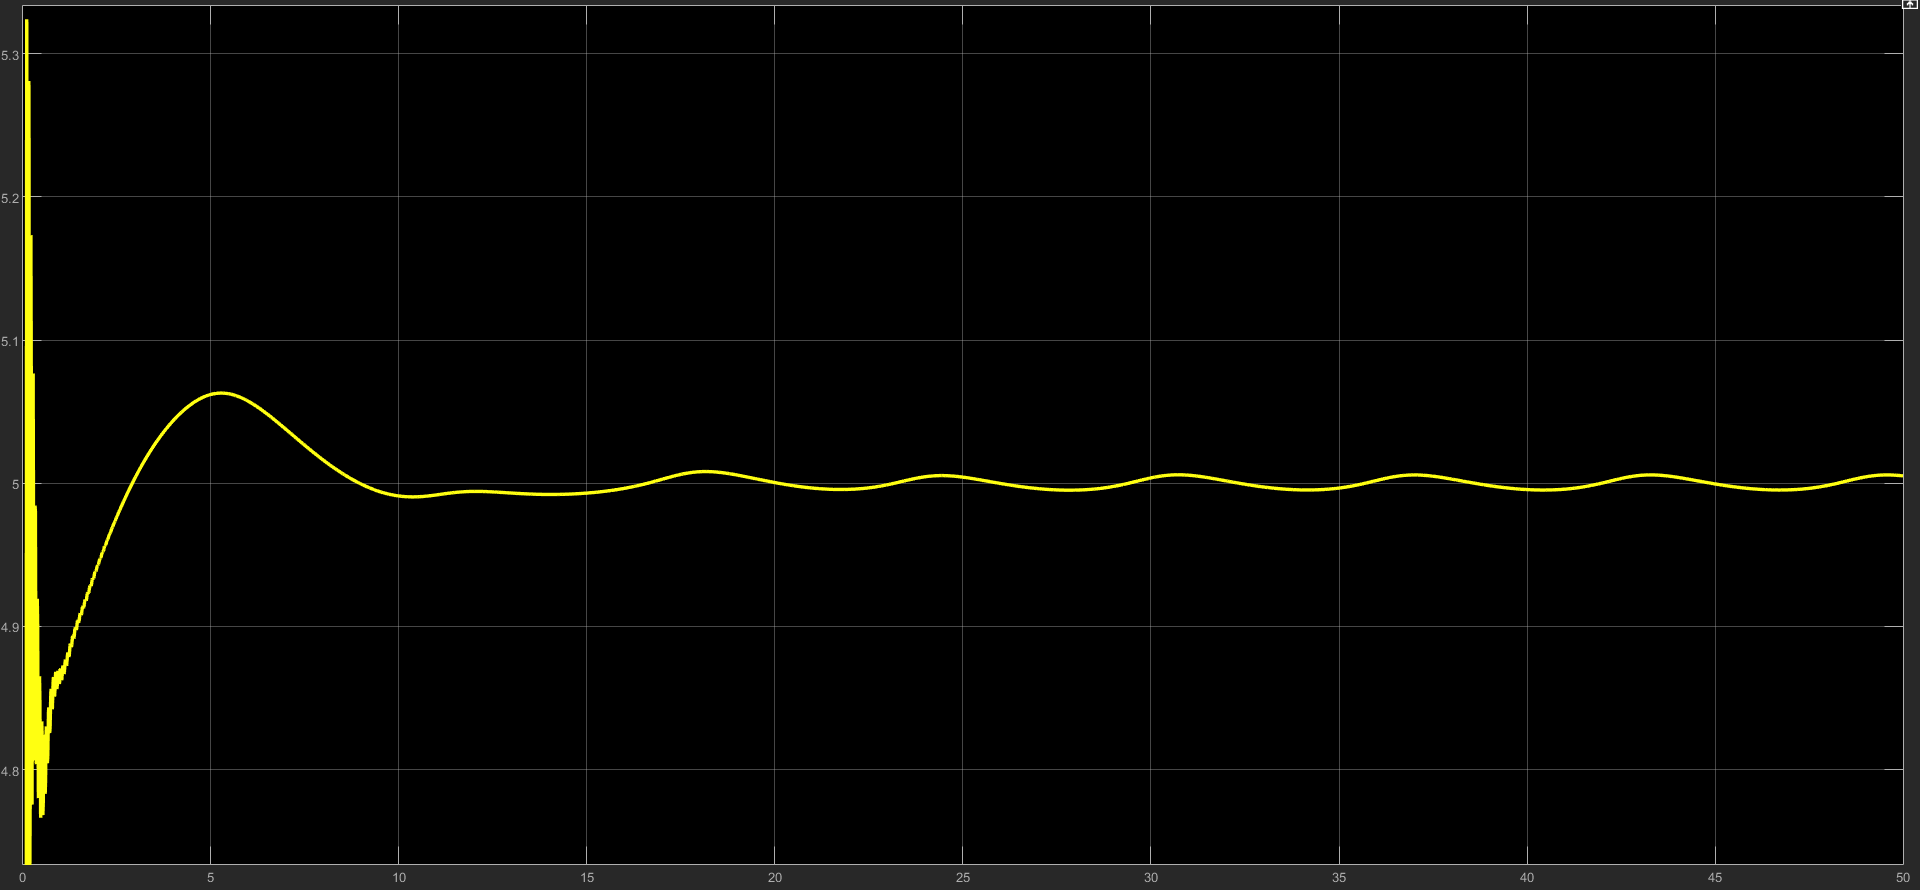
\includegraphics[scale = 0.4]{Q1_5_result.png}
	\caption{خروجی سیستم مقید شده دارای اغتشاش با کنترلر 
		\lr{tube MPC}}
\end{figure}

همانطور که پیداست مقدار فراجهش به حدود 
$0.32$
کاهش پیدا کرده و از این مقدار تغییر محسوسی نمی‌کند. قید اعمال شده به کنترلر بسیار محدود کننده است و باقیمانده فراجهش مربوط به کنترلر 
\lr{PID}
است که با اعمال قید به 
\lr{linear MPC}
نمی‌توان آن را از بین برد.  


\newpage

\section{سوال دوم}
\subsection{بخش اول}

ابتدا سیستم را در سیمولینک شبیه‌سازی می‌کنیم.

 \begin{figure}[h!]
	\centering
	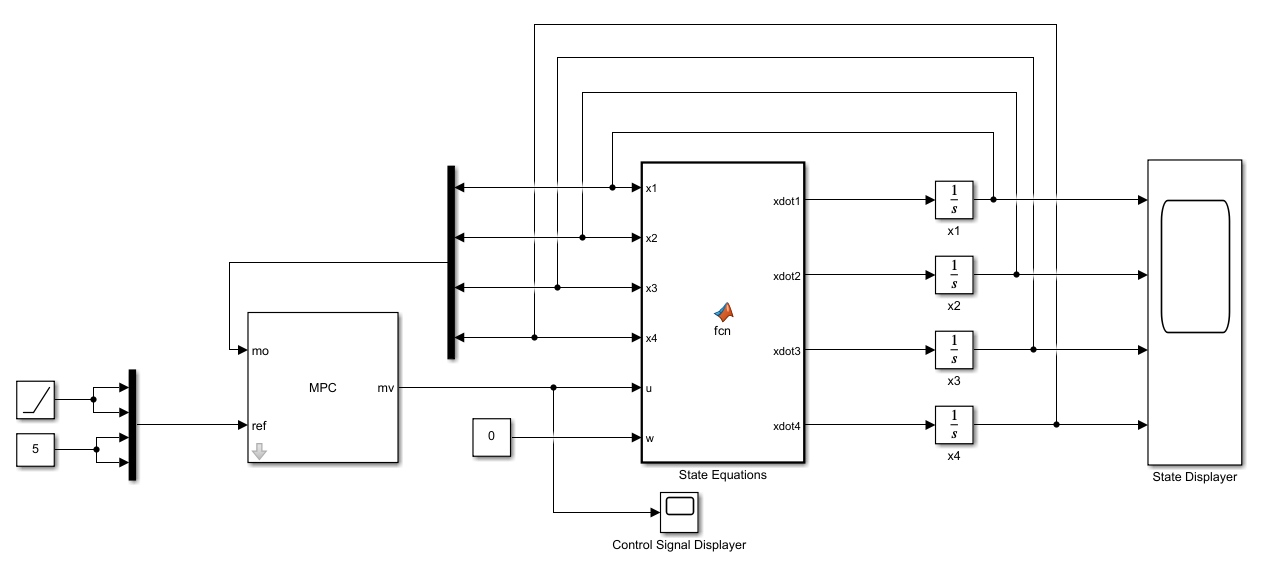
\includegraphics[scale = 0.55]{Q2_1_sim.png}
	\caption{سیستم با کنترلر 
		\lr{linear MPC}}
\end{figure}

با توجه به اینکه در این قسمت اشاره‌ای به اغتشاش نشده بود، مقدار آن را صفر در نظر گرفتیم. رفرنس سرعت‌ها ثابت 5 و رفرنس مکان‌ها با شیب 5 تعریف شده است. معادلات قرار گرفته در 
\lr{Matlab Function}
در ادامه آورده شده است.\\
\begin{latin}
	\begin{lstlisting}[frame=single,numbers=left,style=Matlab-Pyglike]
function [xdot1, xdot2, xdot3, xdot4] = fcn(x1, x2, x3, x4, u, w)

% Parameter Values

m1 = 10000;
m2 = 8000;
k = 500000;
c = 5000;

% State-Equations

xdot1 = x3;
xdot2 = x4;
xdot3 = (1 / m1) * (k * (-x1 + x2) + c * (-x3 + x4) + u + w);
xdot4 = (1 / m2) * (k * (x1 - x2) + c * (x3 - x4));
	\end{lstlisting}
\end{latin}	

\newpage
صفحه مربوط به مقادیر کنترلر در زیر آورده شده است.

 \begin{figure}[h!]
	\centering
	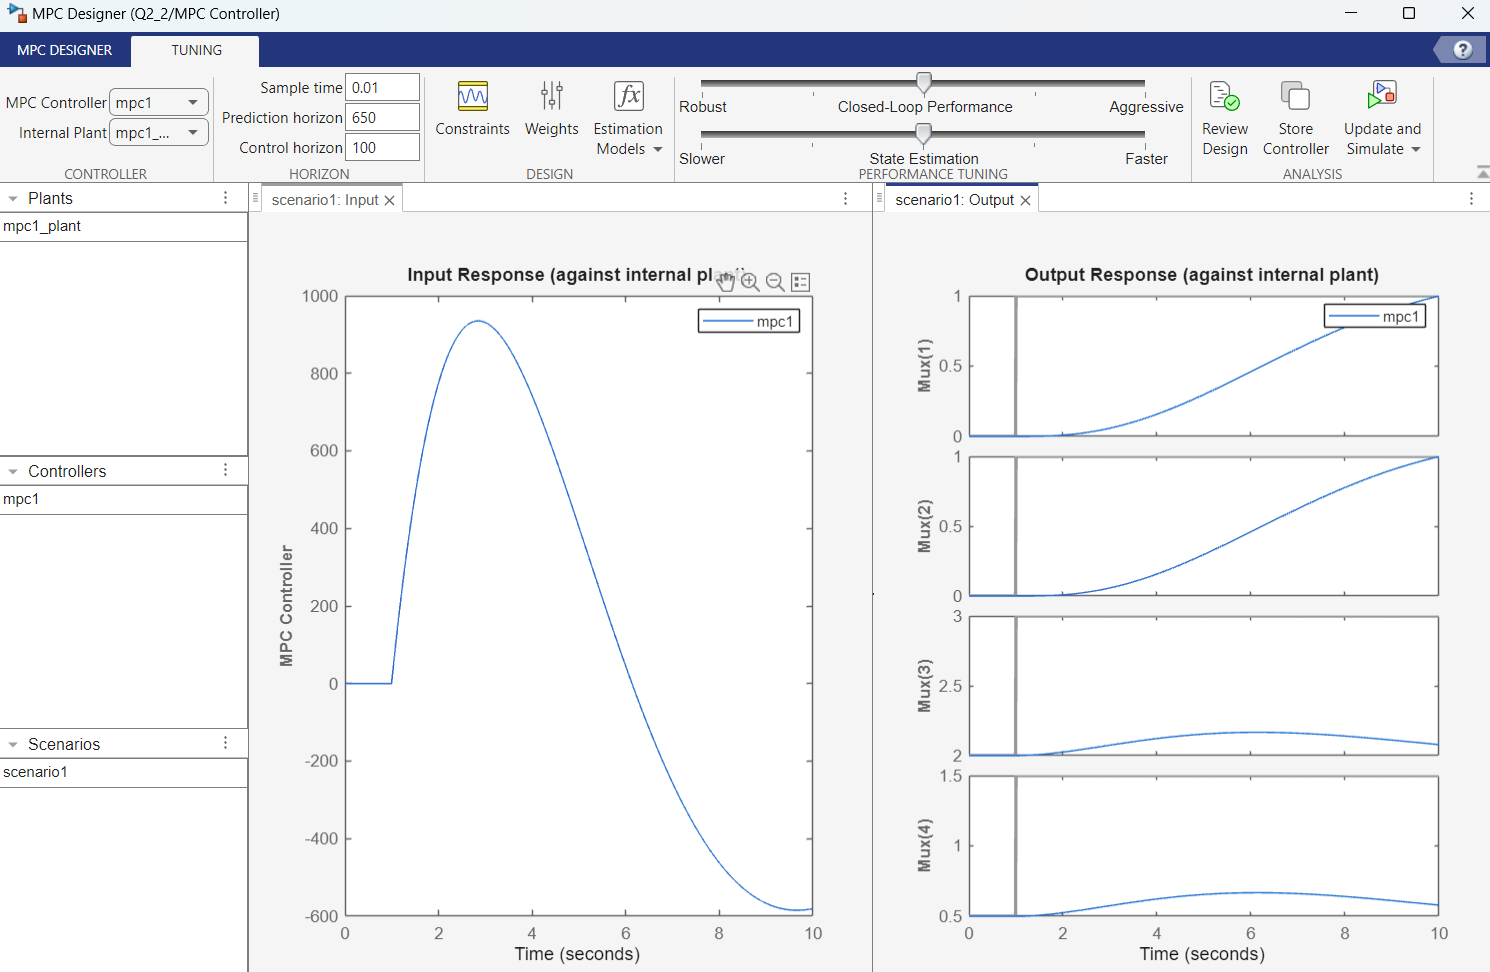
\includegraphics[scale = 0.5]{Q2_1_mpc.png}
	\caption{صفحه مربوط به 
		\lr{linear MPC}}
\end{figure}

وضعیت 
\lr{state}
های سیستم پس از کنترل در ادامه نمابش داده و بررسی می‌شود.
\begin{figure}[h!]
	\centering
	\includegraphics[scale = 0.4]{Q2_1_States.png}
	\caption{خروجی سیستم و وضعیت 
	\lr{state} 
های سیستم}
\end{figure}

همانطور که پیداست،‌ سیستم در حدود 25 تا 30 ثانیه پایدار شده و مقادیر مطلوب را دنبال کرده است.\\
\newpage
سیگنال کنترلی سیستم در ادامه بررسی شده است.
\begin{figure}[h!]
	\centering
	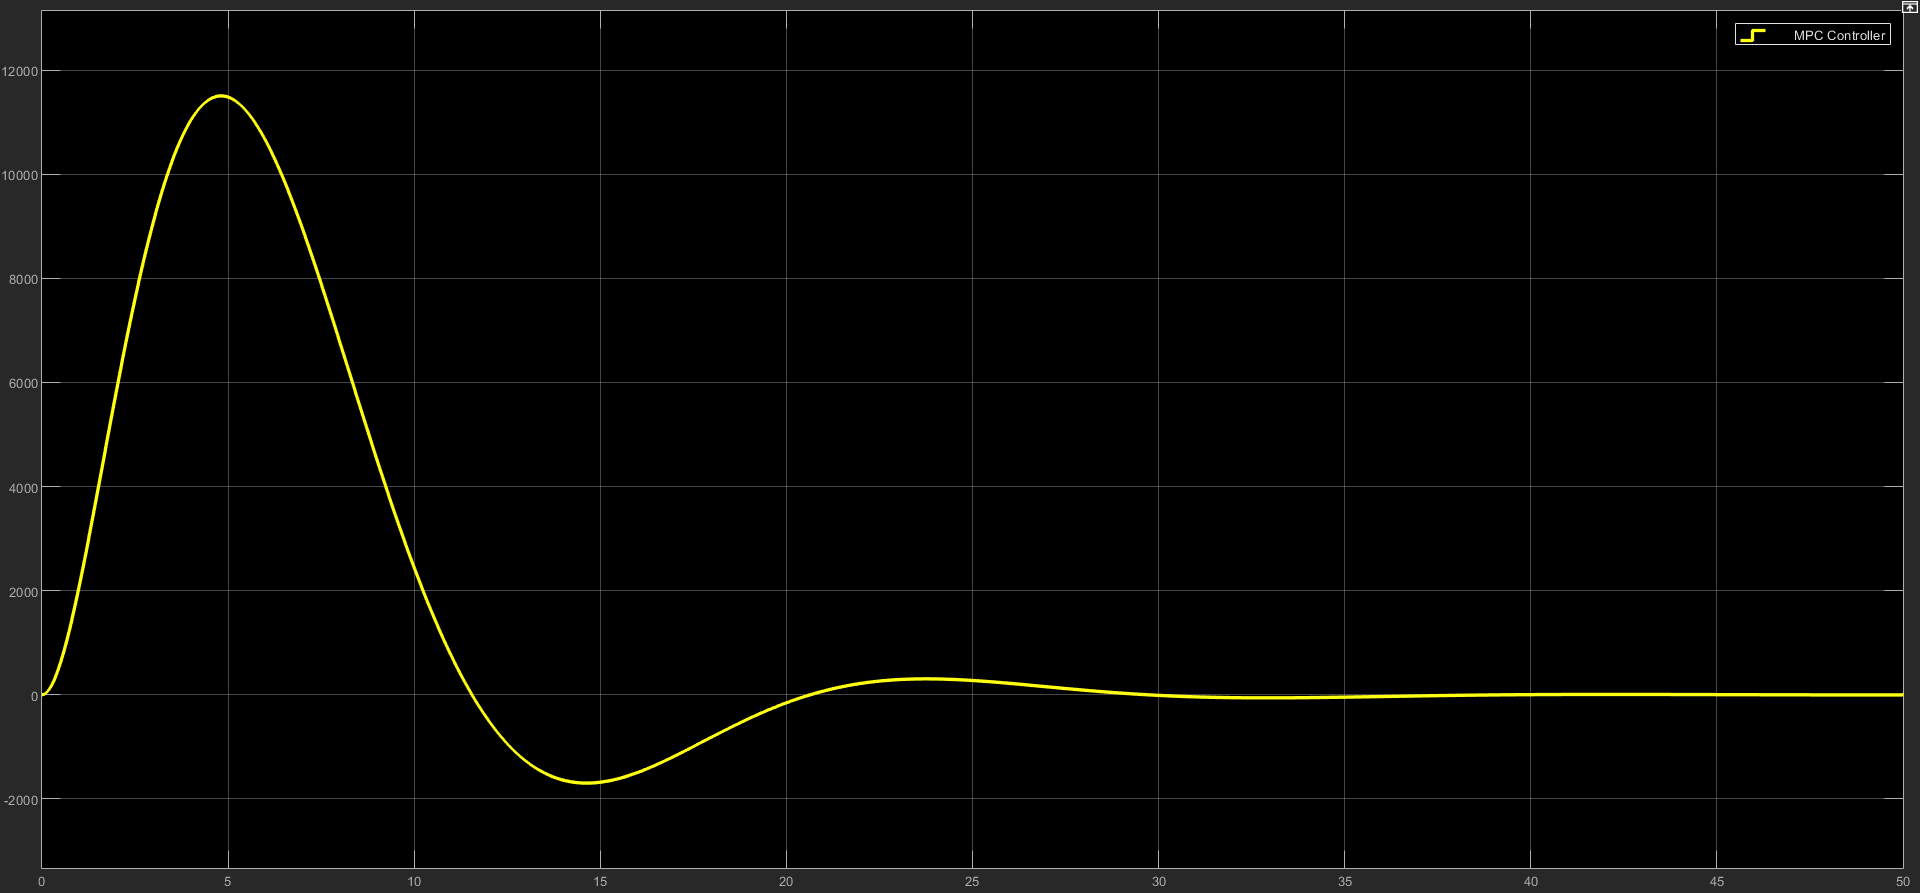
\includegraphics[scale = 0.4]{Q2_1_control.png}
	\caption{سیگنال کنترلی سیستم}
\end{figure}

سیگنال در 5 ثانیه ابتدایی تا مقدار 11500 رفته است که با توجه به بزرگی پارامترهای مسئله،‌ دور از منطق نمی‌باشد. همچنین پس از پایداری سیستم، سیگنال به صفر متمایل شده که طبیعی می‌باشد.

\newpage
\subsection{بخش دوم}
در این قسمت به بررسی تاثیر اعمال قید روی کنترلر می‌پردازیم.
\subsubsection{قید نرم}
ابتدا قید 
$x_4 \leq 1.5$
را به صورت نرم به کنترلر اضافه می‌کنیم. پارامترهای کنترلر تغییری نمی‌کنند.

\begin{figure}[h!]
	\centering
	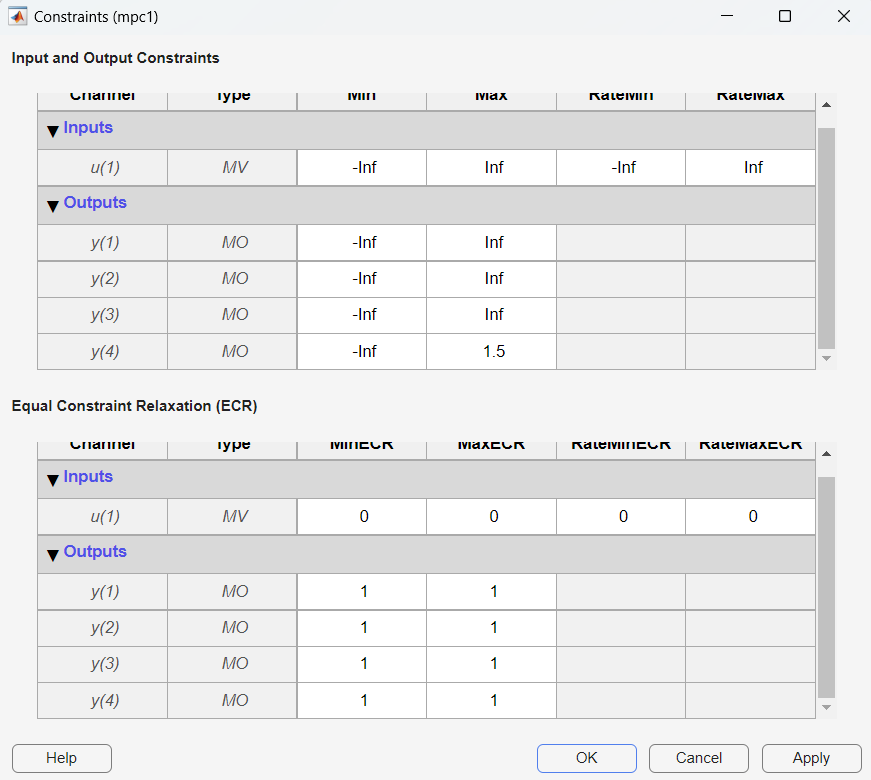
\includegraphics[scale = 0.5]{Q2_2_1_cons.png}
	\caption{صفحه مربوط به قید نرم 
		\lr{linear MPC}}
\end{figure}

در ادامه سیگنال کنترلی و خروجی‌های سیستم را بررسی می‌کنیم.

 \begin{figure}[h!]
	\centering
	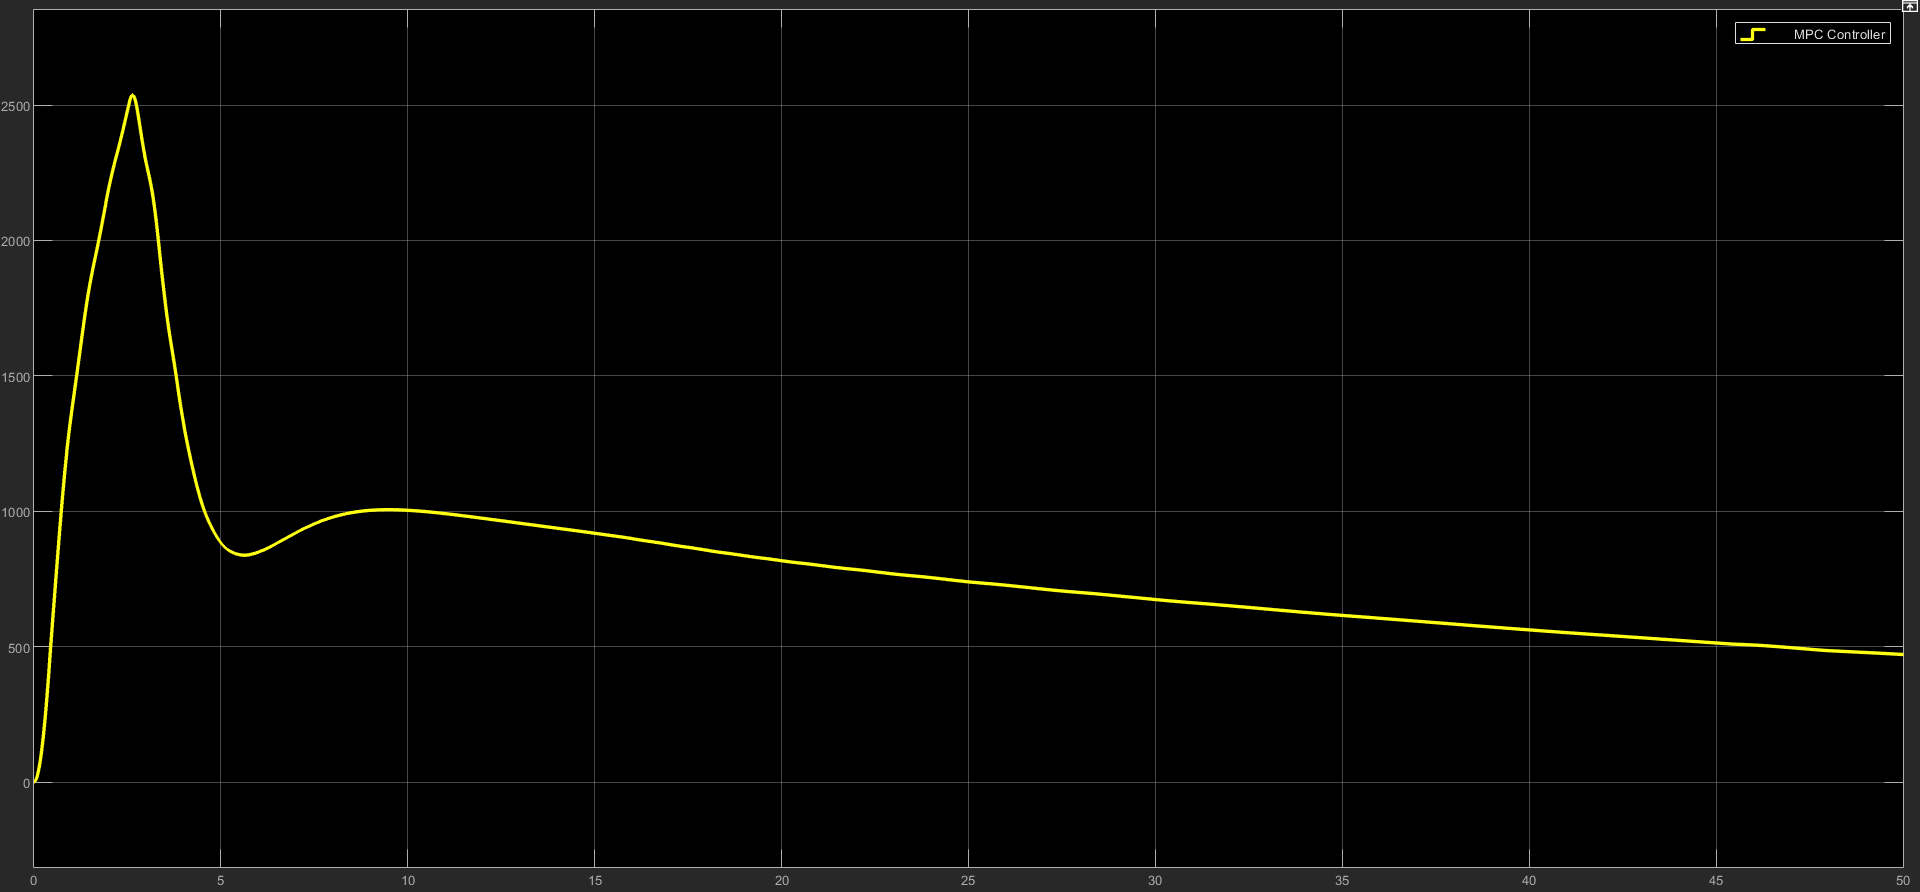
\includegraphics[scale = 0.3]{Q2_2_1_control.png}
	\caption{سیگنال کنترلی پس از اعمال قید نرم روی کنترلر}
\end{figure}

سیگنال کنترلی پس از رسیدن به حدود 2500 که بسیار کمتر حالت قبل است، به پایین برگشته و با مقدار کم و شیب کم به سمت صفر شدن حرکت می‌کند. 

\newpage
\begin{figure}[h!]
	\centering
	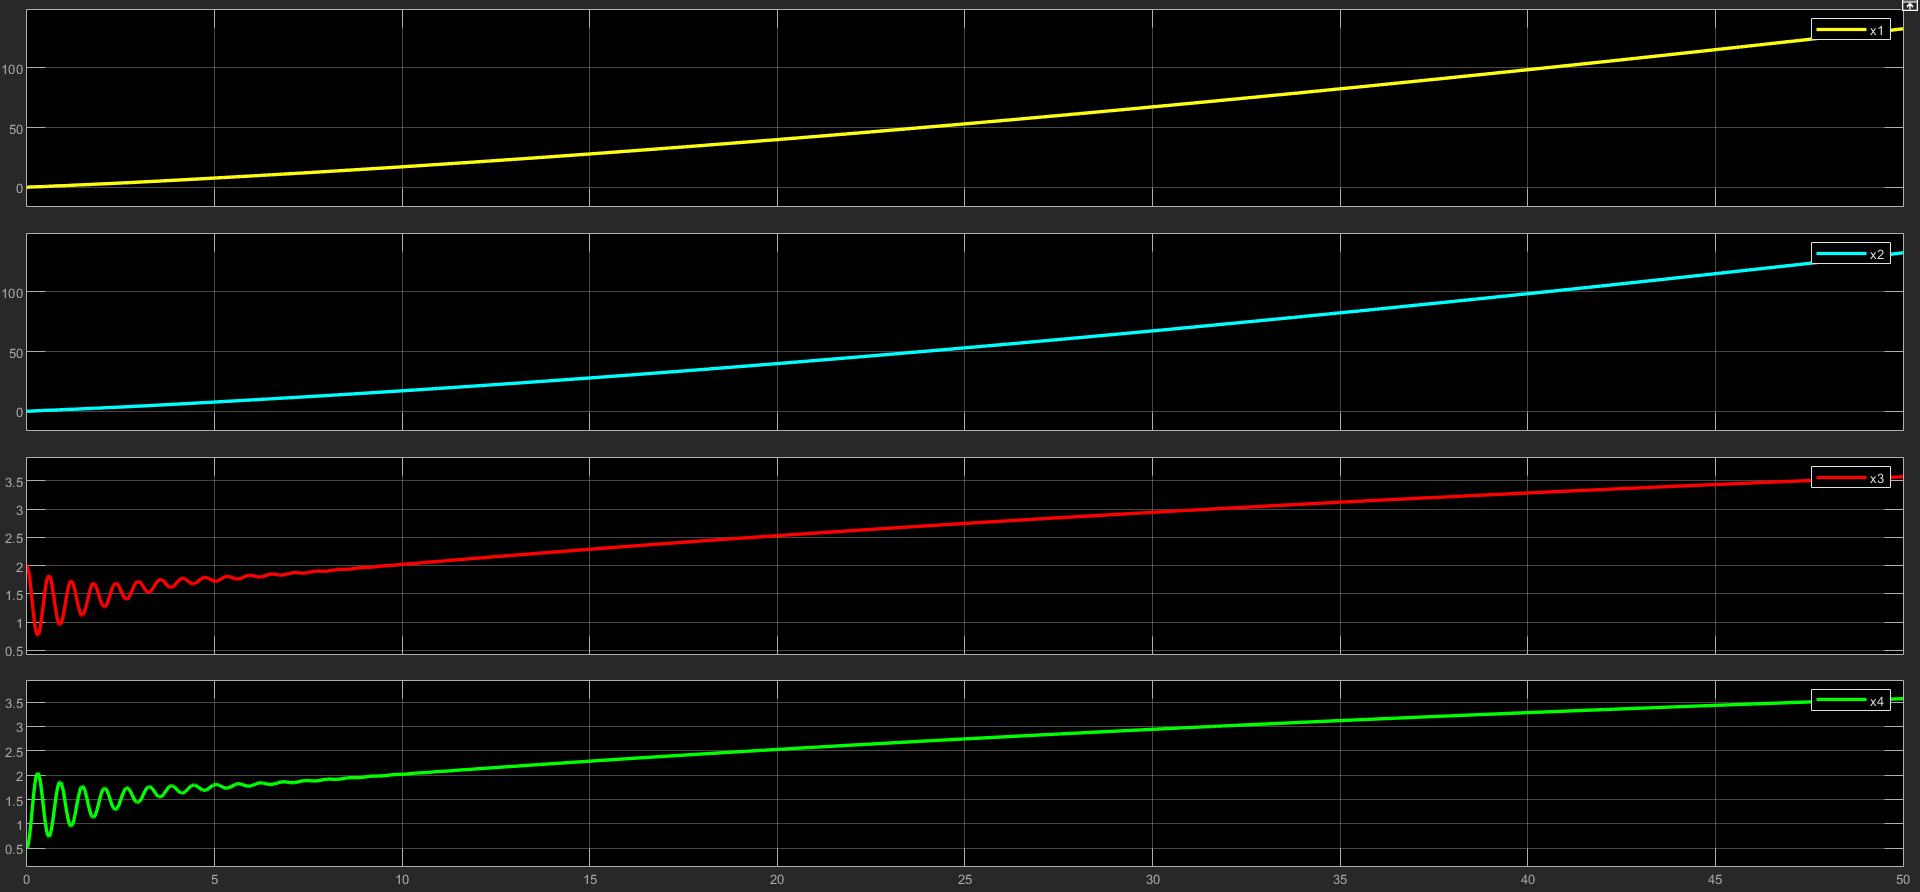
\includegraphics[scale = 0.3]{Q2_2_1_states.png}
	\caption{وضعیت 
		\lr{state}
		ها پس از اعمال قید نرم روی کنترلر}
\end{figure}

\lr{state}
های سیستم با سرعت بسیار کمتری نسبت به حالت بدون قید در حال رسیدن به مقدار رفرنس‌ها هستند.\\
همانطور که مشاهده شد، با اعمال قید به صورت نرم،‌ سیستم به شدت کند شده و حتی با گذر 50 ثانیه هم نتوانسته به مقدار رفرنس برسد. چون قید به صورت نرم بود، سیستم از قید عبور کرده و عملا قید فقط باعث کندی سیستم شده است.



\subsubsection{قید سخت}
حال با تغییر مقدار 
\lr{ECR}
مربوط به قید چهارم، آن را به صورت سخت به سیستم اعمال می‌کنیم. 

\begin{figure}[h!]
	\centering
	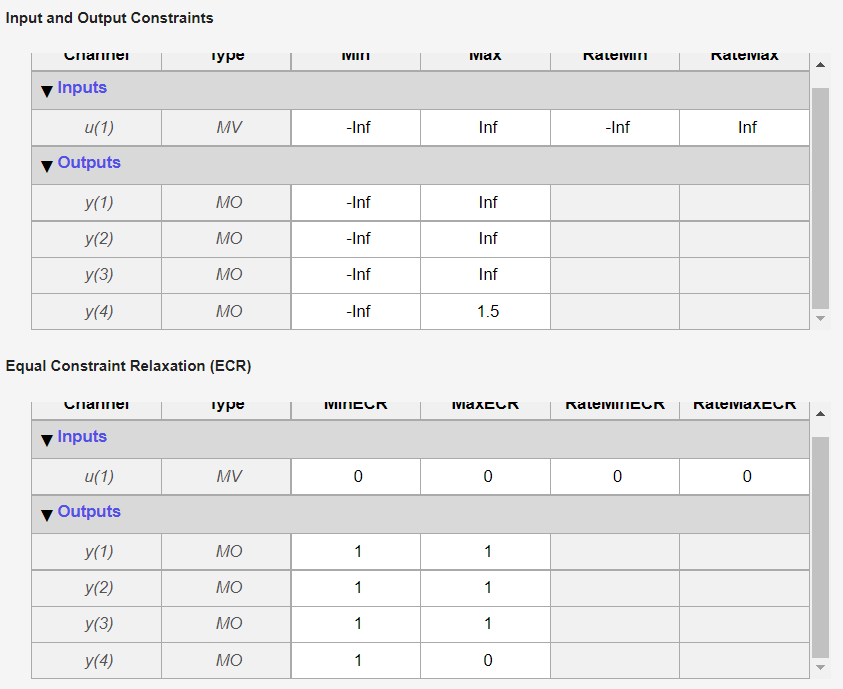
\includegraphics[scale = 0.5]{Q2_2_2_cons.png}
	\caption{صفحه مربوط به قید سخت 
		\lr{linear MPC}}
\end{figure}

در ادامه سیگنال کنترلی و خروجی‌های سیستم را بررسی می‌کنیم.
\newpage

\begin{figure}[h!]
	\centering
	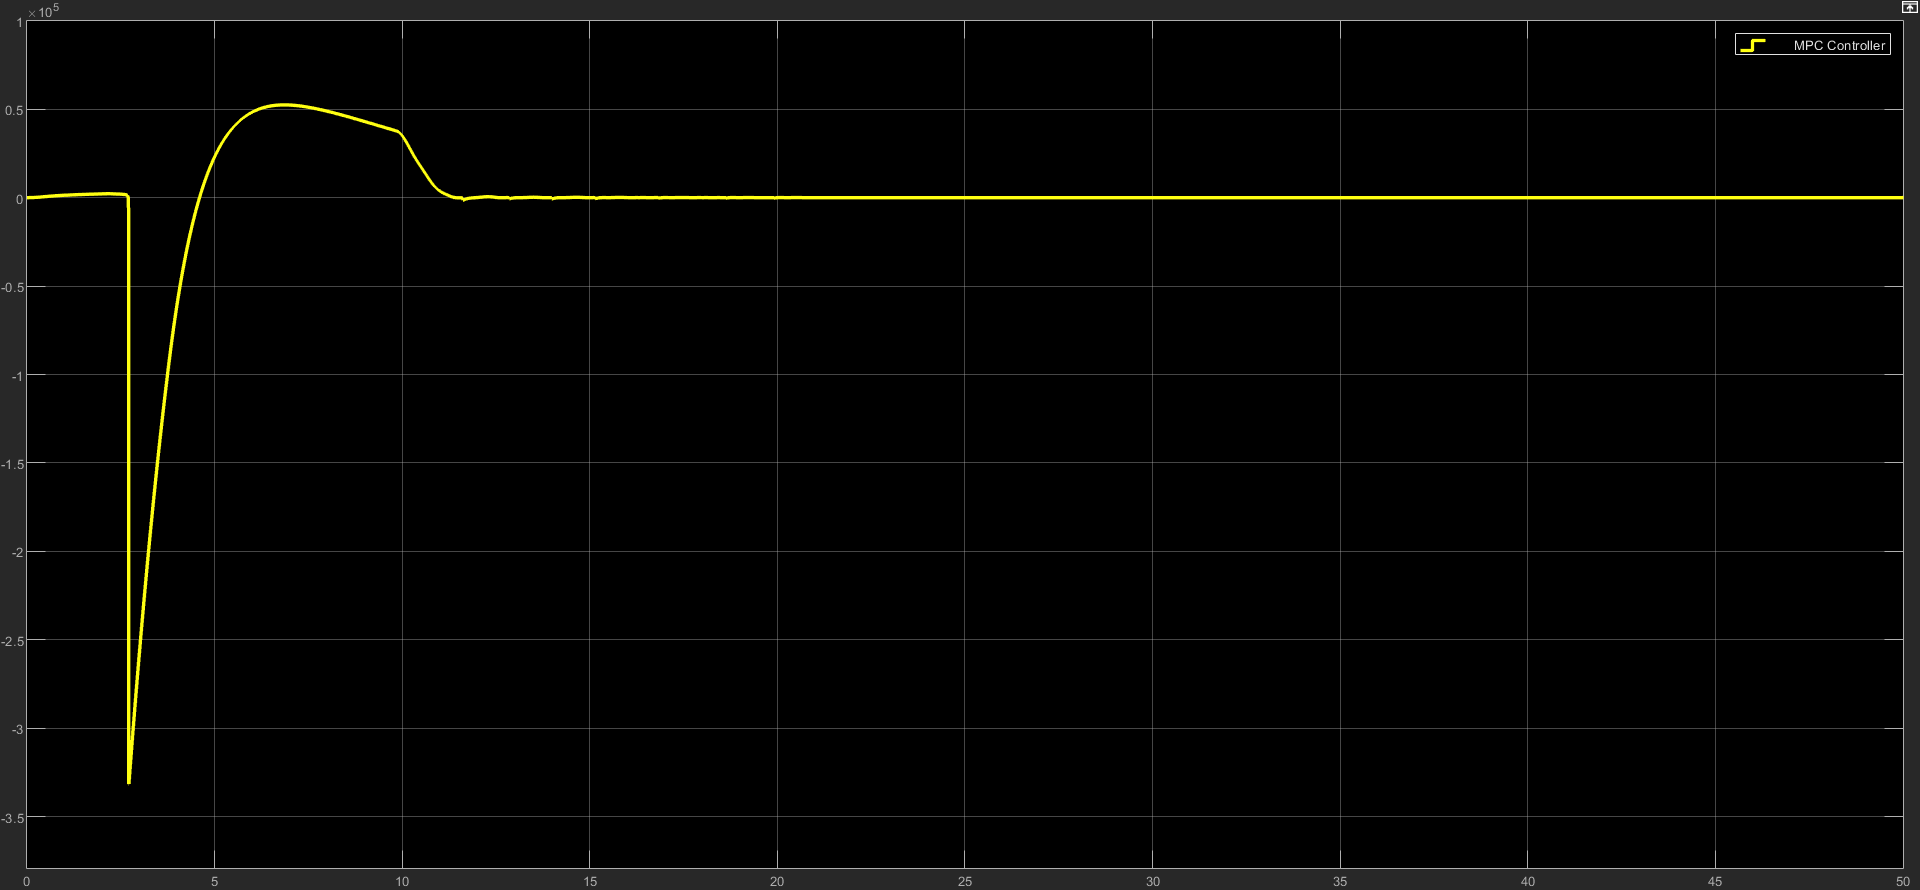
\includegraphics[scale = 0.3]{Q2_2_2_control.png}
	\caption{سیگنال کنترلی پس از اعمال قید سخت روی کنترلر}
\end{figure}

با توجه به عبور 
$x_4$
از قید سخت در ابتدای حرکت، کنترلر با اعمال سیگنال منفی با بزرگی بسیار زیاد(حدود 330000)، سعی می‌کند تا قید خواسته شده را رعایت کند.
\begin{figure}[h!]
	\centering
	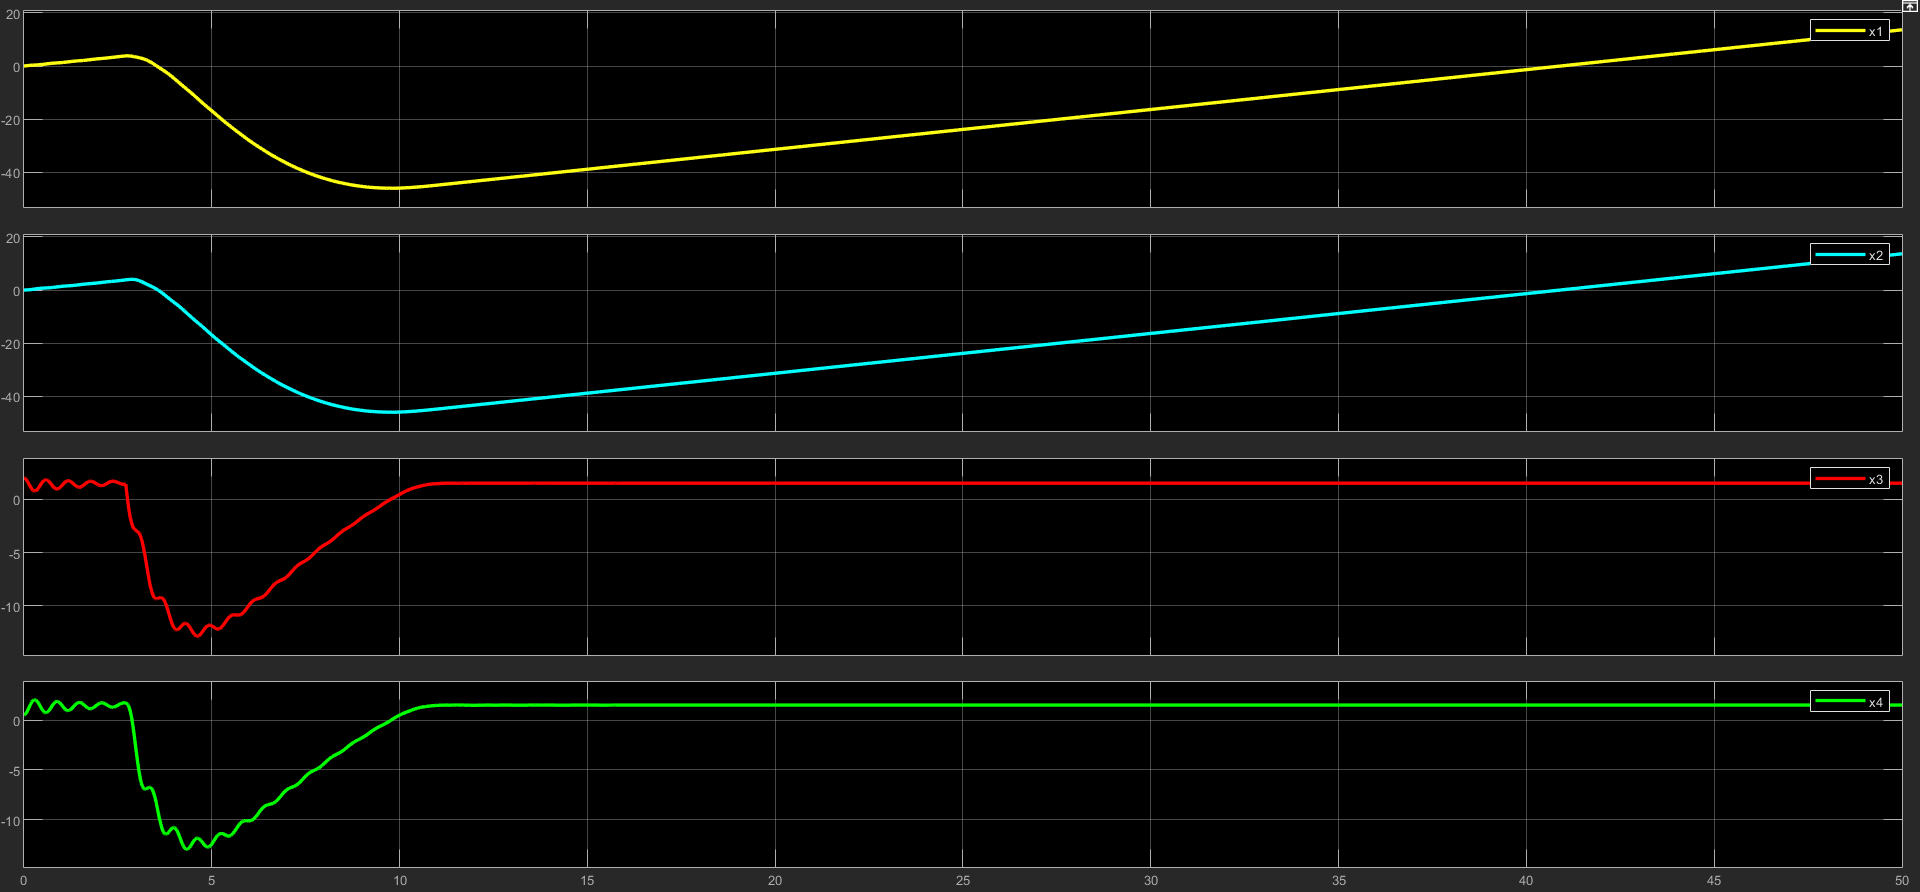
\includegraphics[scale = 0.3]{Q2_2_2_states.png}
	\caption{وضعیت 
		\lr{state}
		ها پس از اعمال قید سخت روی کنترلر}
\end{figure}

پس از عبور از سرعت
$1.5$
 در ابتدای حرکت و دربافت سیگنال منفی از کنترلر، سرعت‌ها تا حدود 
$-13$
کاهش بافته‌اند تا پس از آن بتوانند قید خواسته شده را رعایت کنند. همانطور که مشخص است،‌ سیستم در حدود 11 ثانیه به قید رسیده و پایدار شده است.\\
به عنوان نتیجه می‌توان گفت قید نرم صرفا باعث کندی سیستم شده ولی قید سخت، سیستم را در مقدار مشخص شده مقید می‌کند.

\newpage
\subsection{بخش سوم}

اغتشاش را به سیستم اعمال می‌کنیم.
 \begin{figure}[h!]
	\centering
	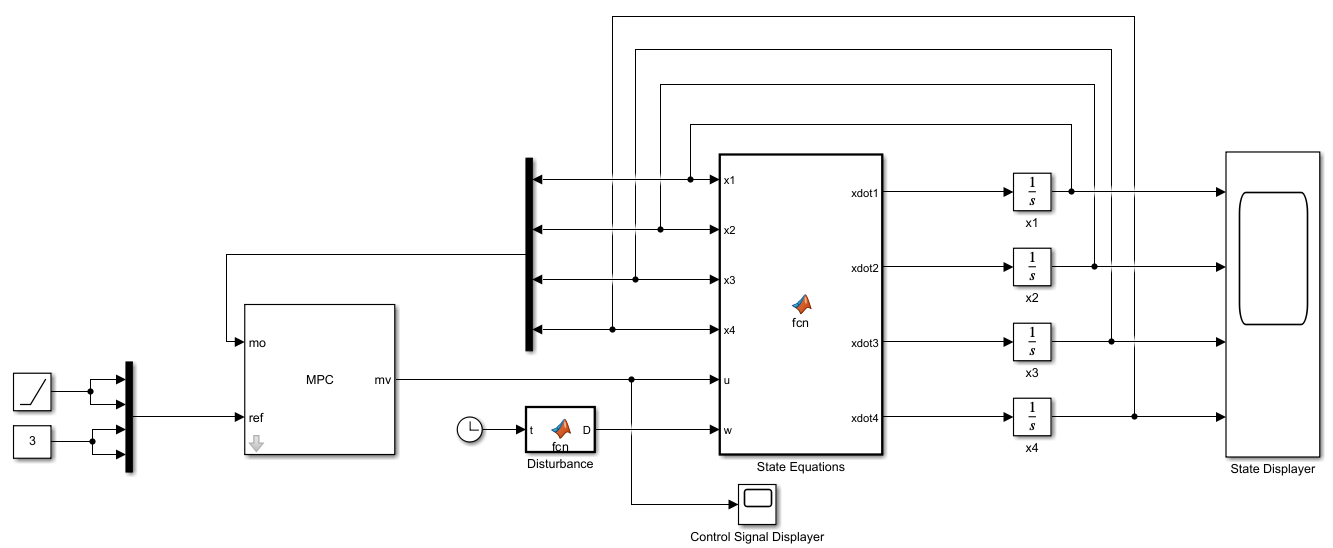
\includegraphics[scale = 0.55]{Q2_3_sim.png}
	\caption{سیستم دارای اغتشاش با کنترلر 
		\lr{linear MPC}}
\end{figure}

وضعیت 
\lr{state}
ها و سیگنال کنترلی در ادامه بررسی می‌شوند.

\begin{figure}[h!]
	\centering
	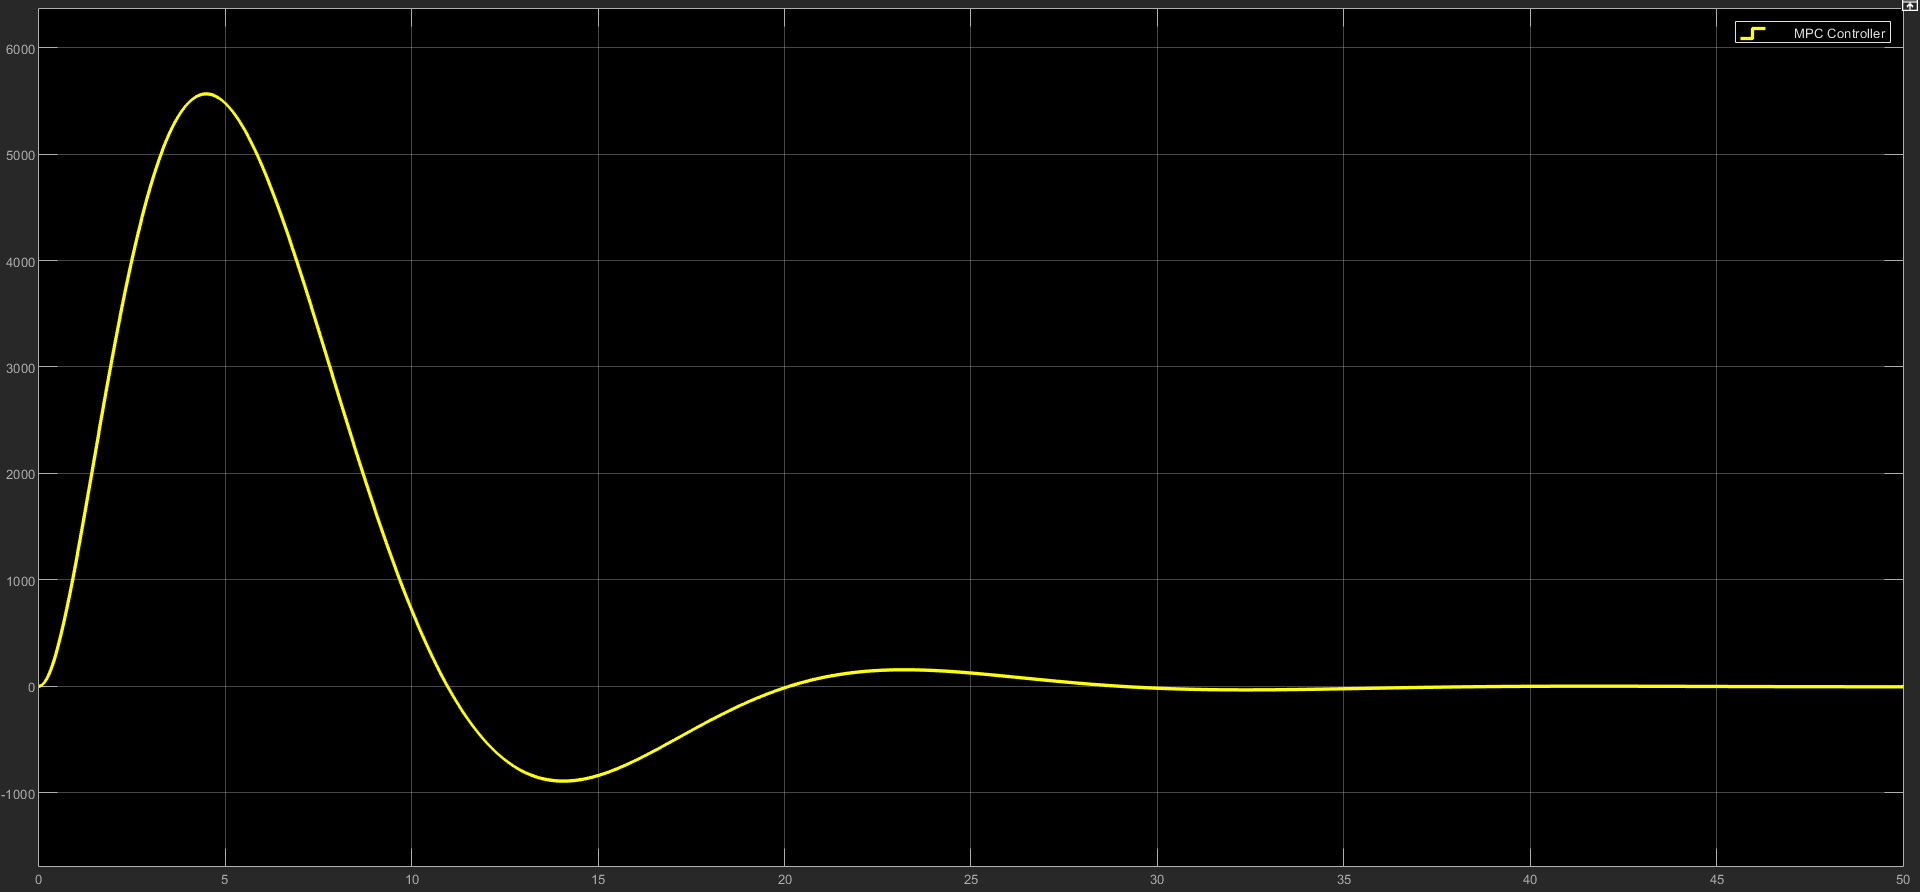
\includegraphics[scale = 0.4]{Q2_3_1_control.png}
	\caption{سیگنال کنترلی پس از اعمال اغتشاش با کنترلر 
	\lr{linear MPC}}
\end{figure}

تنها تفاوت محسوس آن به علت تغییر مقدار رفرنس از 5 به 3 می‌باشد.

\newpage
\begin{figure}[h!]
	\centering
	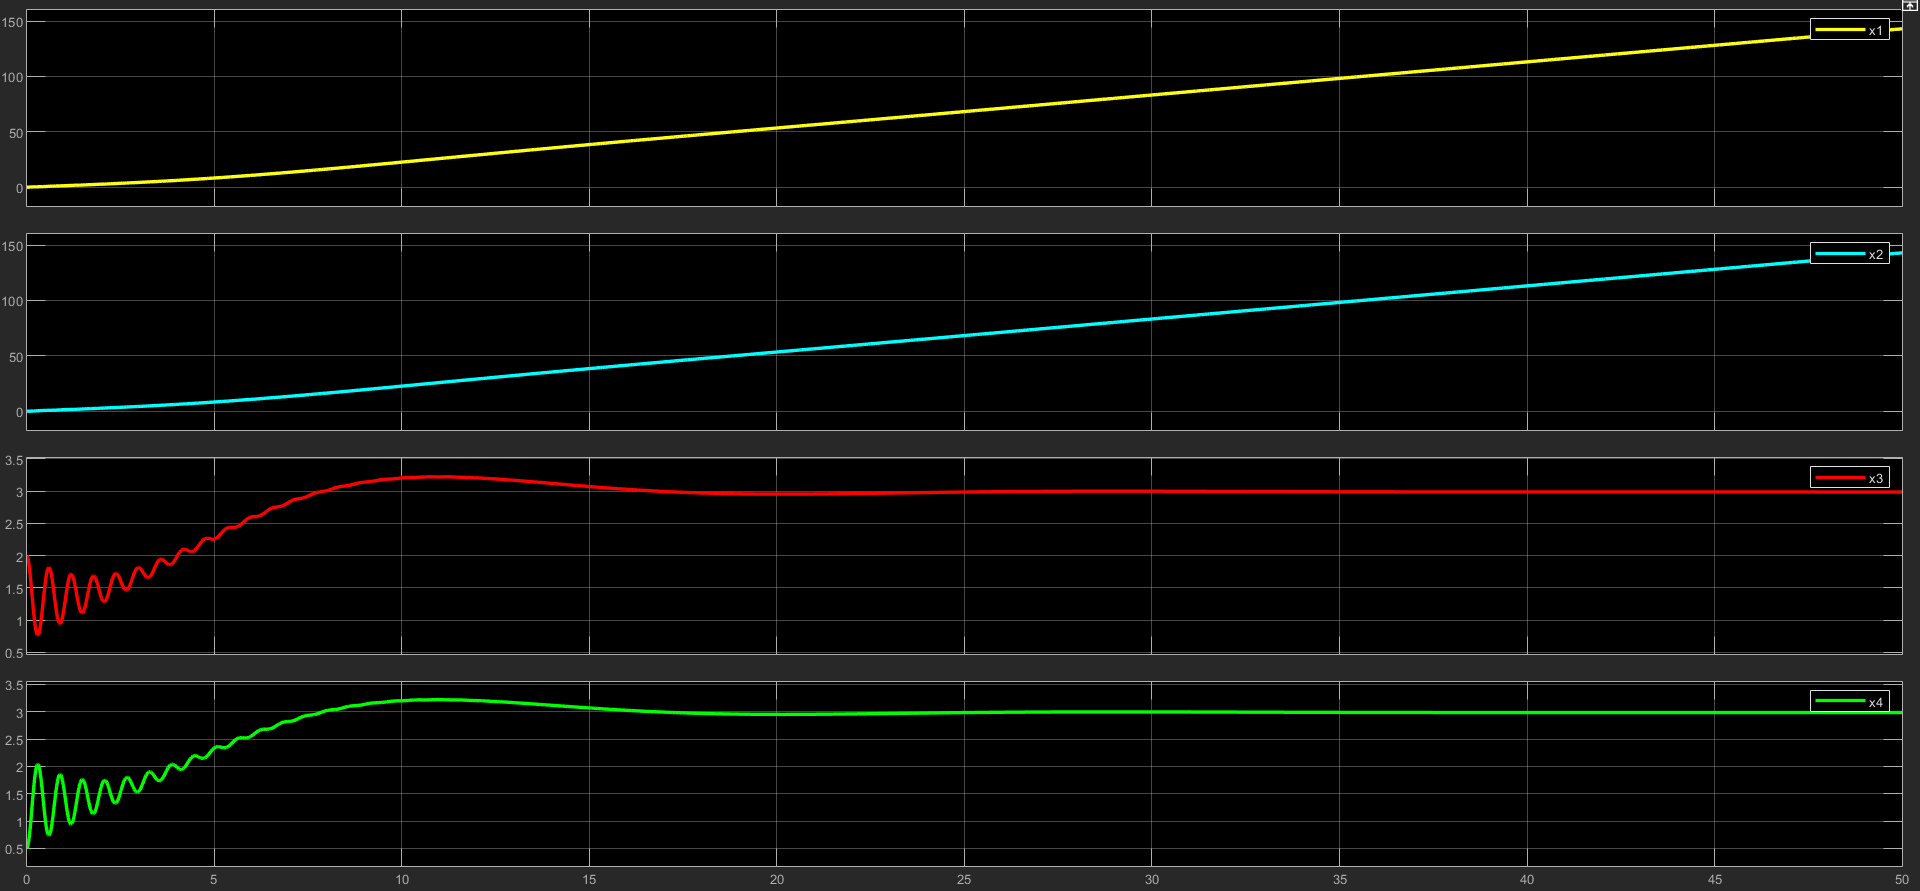
\includegraphics[scale = 0.4]{Q2_3_1_states1.png}
	\caption{وضعیت 
		\lr{state}
		ها پس از اعمال اغتشاش به سیستم با کنترلر 
	\lr{linear MPC}}
\end{figure}

با توجه به کوچک بودن بیش از حد مقدار اغتشاش، تصویر زوم شده را هم نمایش می‌دهیم.
\begin{figure}[h!]
	\centering
	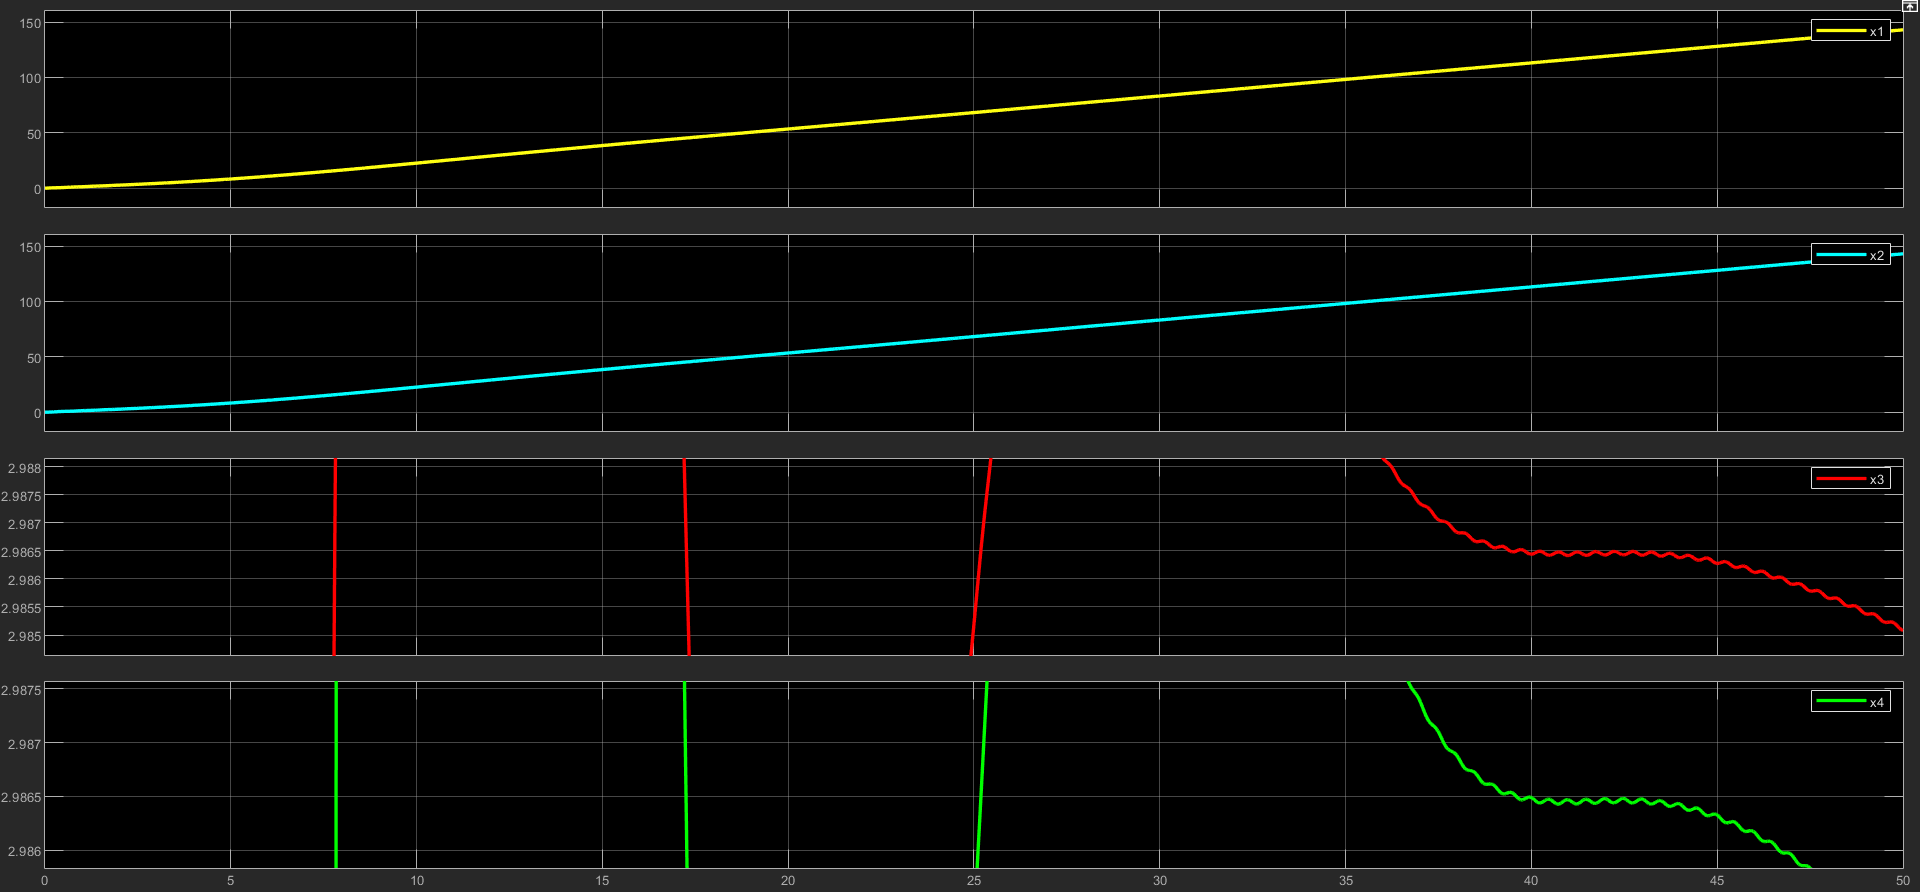
\includegraphics[scale = 0.4]{Q2_3_1_states2.png}
	\caption{وضعیت 
		\lr{state}
		ها پس از اعمال اغتشاش به سیستم با کنترلر 
		\lr{linear MPC}}
\end{figure}

همانطور که مشاهده می‌شود،‌ یک نوسان بسیار کوچک به سرعت‌ها وارد شده است.

\newpage

با توجه به کوچکی اغتشاش، نمایش تغییرات پس از اعمال کنترلر جدید بسیار مشکل است بنابراین بجای اغتشاش داده شده در سوال، از 
$D = 2000sin(4\pi t)$
استفاده می‌کنیم. درنتیجه خواهیم داشت:
\begin{figure}[h!]
	\centering
	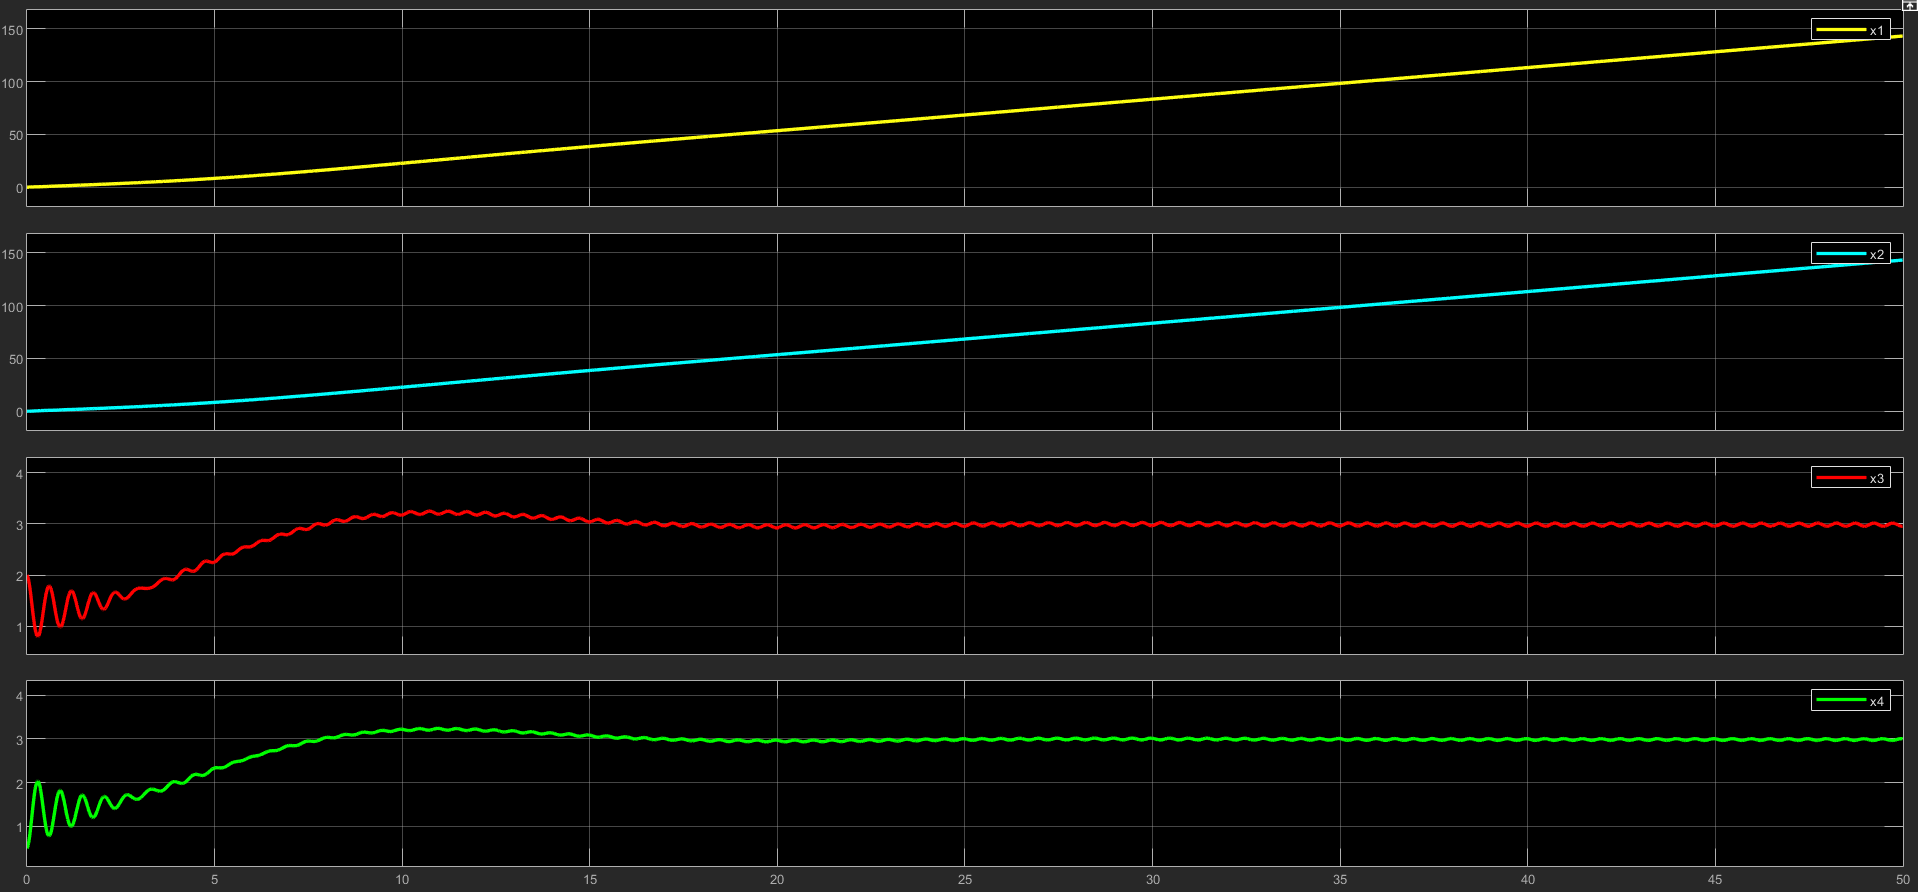
\includegraphics[scale = 0.4]{Q2_3_1_states1D.png}
	\caption{وضعیت 
		\lr{state}
		ها پس از اعمال اغتشاش بزرگتر به سیستم با کنترلر 
		\lr{linear MPC}}
\end{figure}

\begin{figure}[h!]
	\centering
	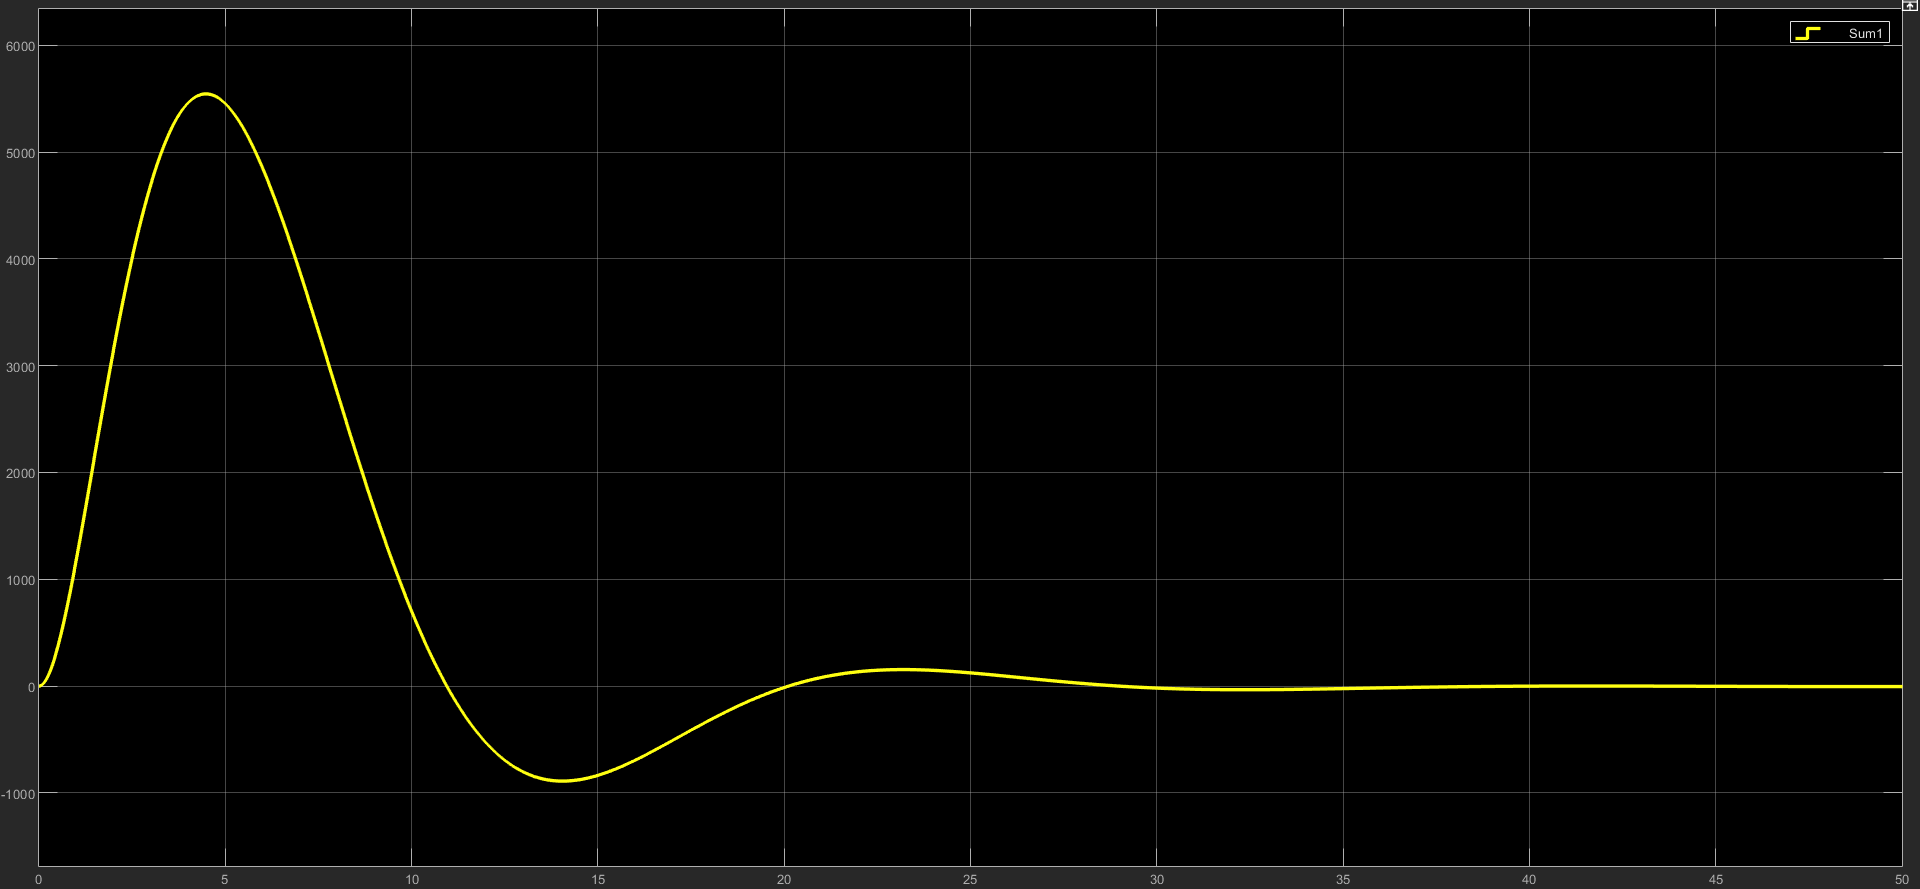
\includegraphics[scale = 0.4]{Q2_3_1_controlD.png}
	\caption{سیگنال کنترلی پس از اعمال اغتشاش بزرگتر با کنترلر 
		\lr{linear MPC}}
\end{figure}

\newpage

حال سعی می‌کنیم با اضافه کردن کنترلر 
\lr{PID}
و استفاده از کنترل 
\lr{tube MPC}
اثر اغتشاش را کاهش دهیم.
\begin{figure}[h!]
	\centering
	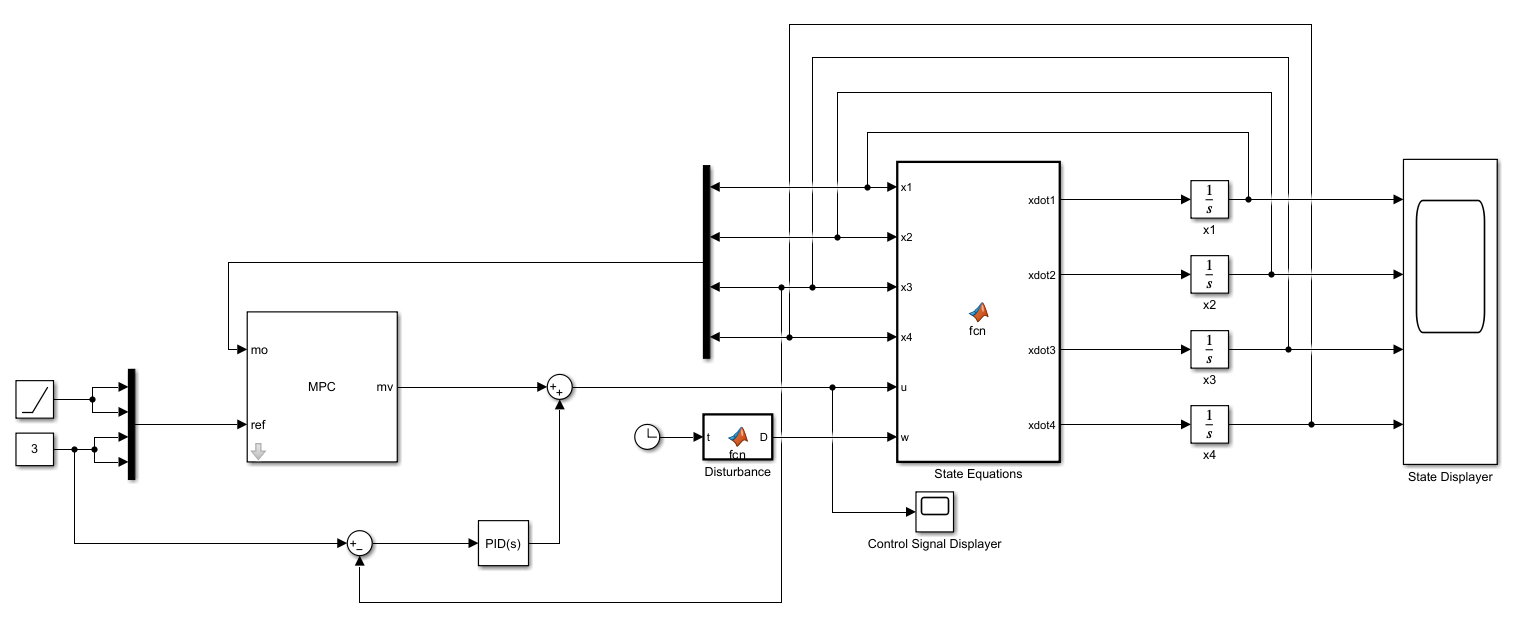
\includegraphics[scale = 0.5]{Q2_3_1_sim.png}
	\caption{سیستم دارای اغتشاش با کنترلر 
		\lr{tub MPC}}
\end{figure}

ضرایب 
\lr{PID}
به دست آمده در تصویر زیر قابل مشاهده است.
\begin{figure}[h!]
	\centering
	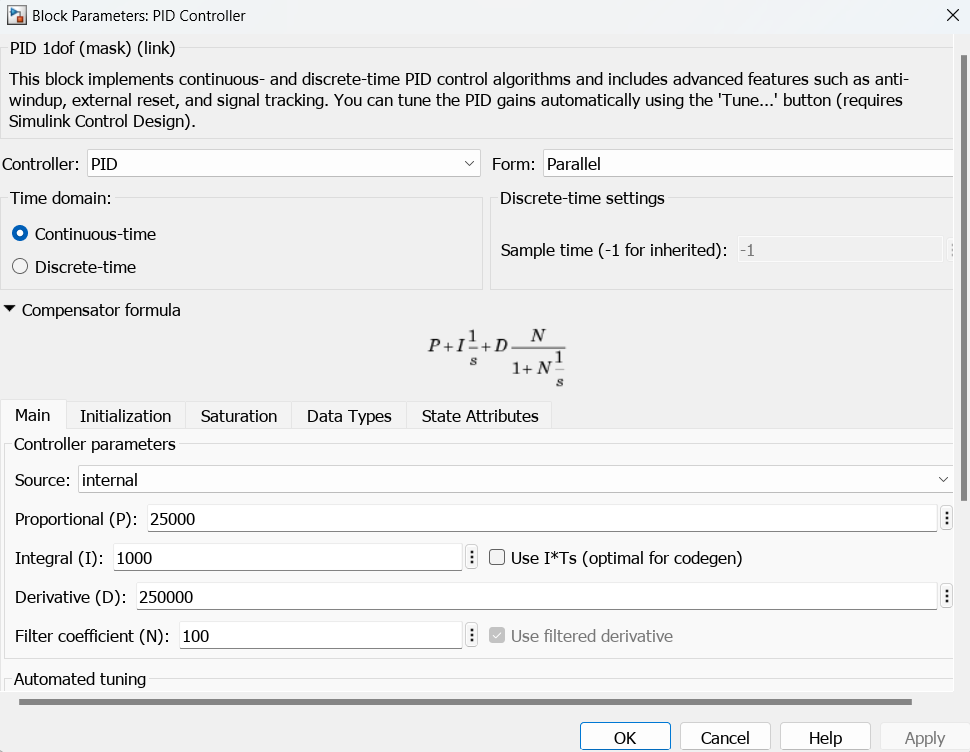
\includegraphics[scale = 0.5]{Q2_3_2_pid.png}
	\caption{ضرایب 
		\lr{PID}
		به کار رفته در 
		\lr{tub MPC}}
\end{figure}

\newpage
در ادامه سیگنال کنترلی و خروجی‌های سیستم با اغتشاش و کنترلر 
\lr{tube MPC}
 را بررسی می‌کنیم.
\begin{figure}[h!]
	\centering
	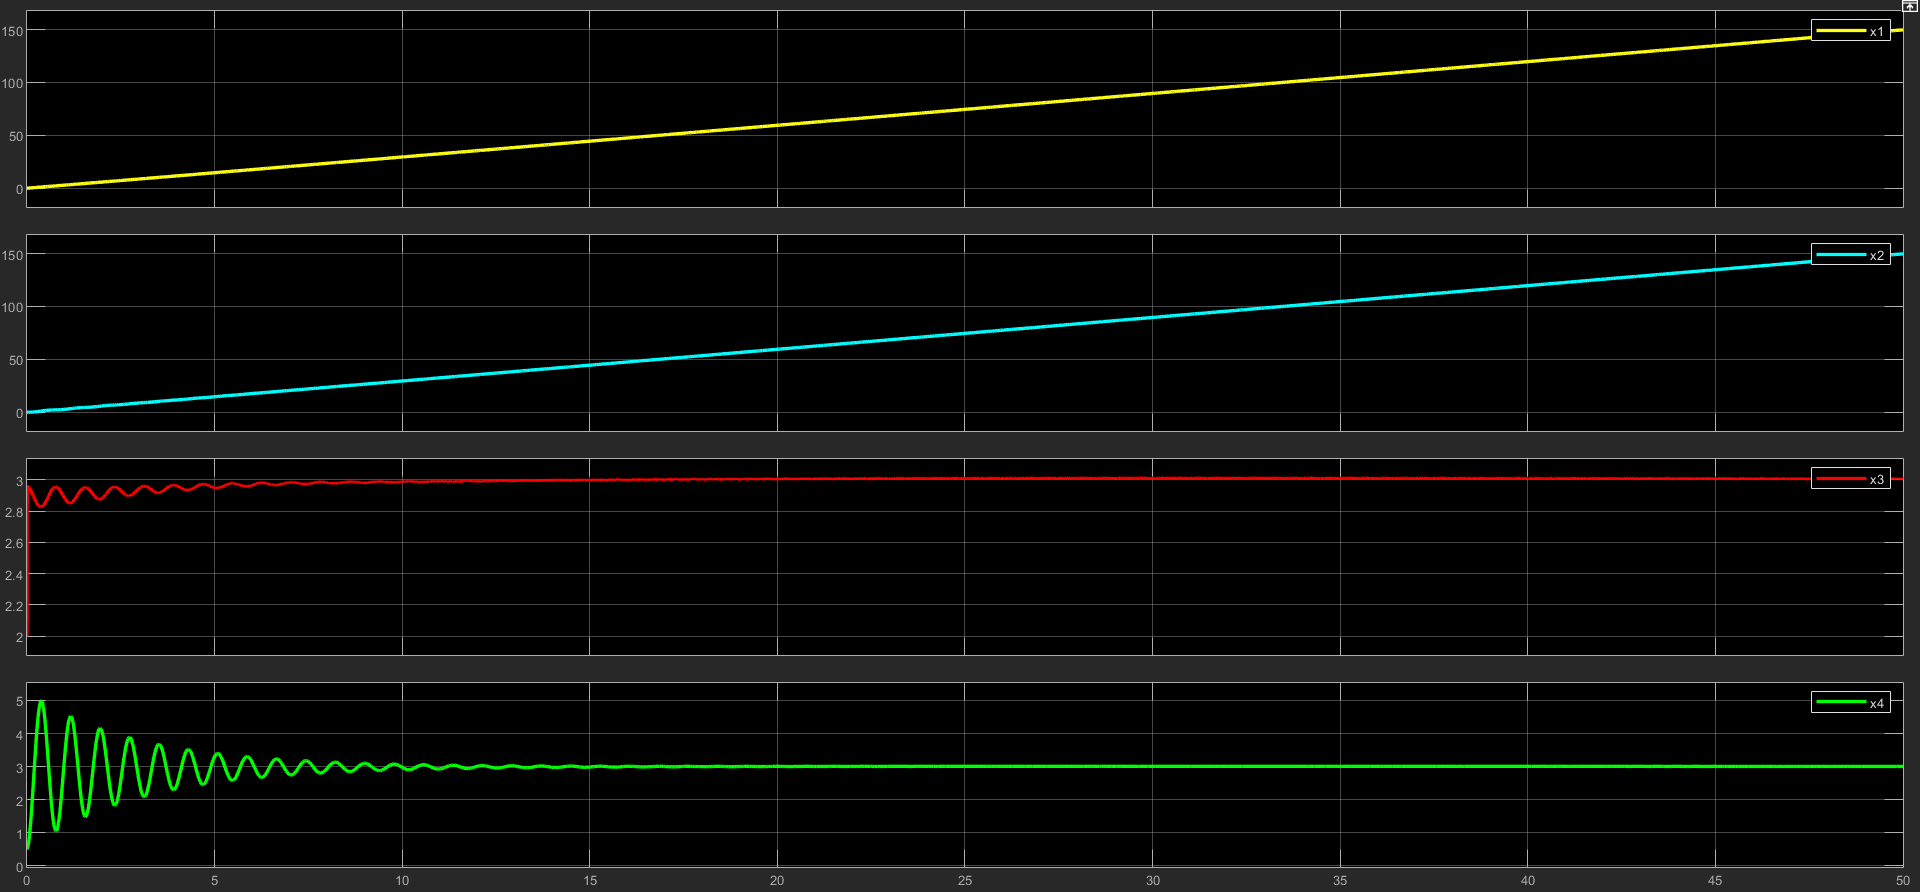
\includegraphics[scale = 0.4]{Q2_3_2_states1D.png}
	\caption{وضعیت 
		\lr{state}
		ها پس از اعمال اغتشاش بزرگتر به سیستم با کنترلر 
		\lr{tube MPC}}
\end{figure}

\begin{figure}[h!]
	\centering
	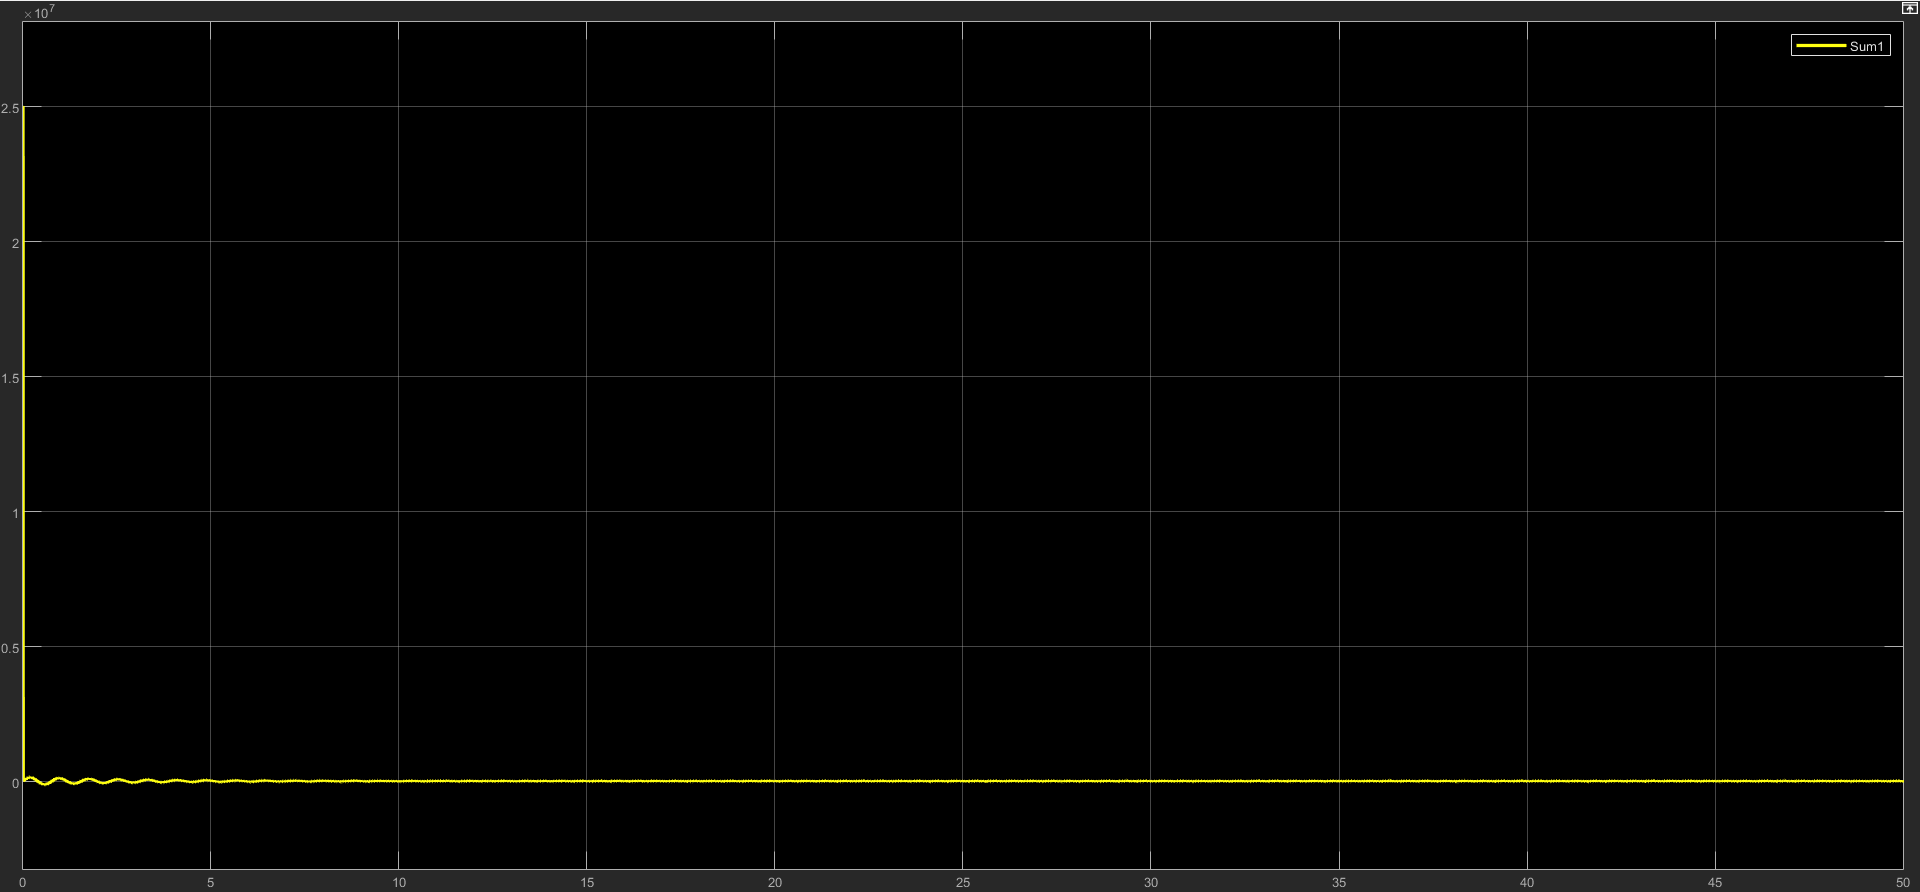
\includegraphics[scale = 0.4]{Q2_3_2_control1.png}
	\caption{سیگنال کنترلی پس از اعمال اغتشاش بزرگتر با کنترلر 
		\lr{tube MPC}}
\end{figure}

\newpage
همچنین سیگنال کنترلی با زوم بیشتر جهت نمایش بهتر قرار می‌گیرد.
\begin{figure}[h!]
	\centering
	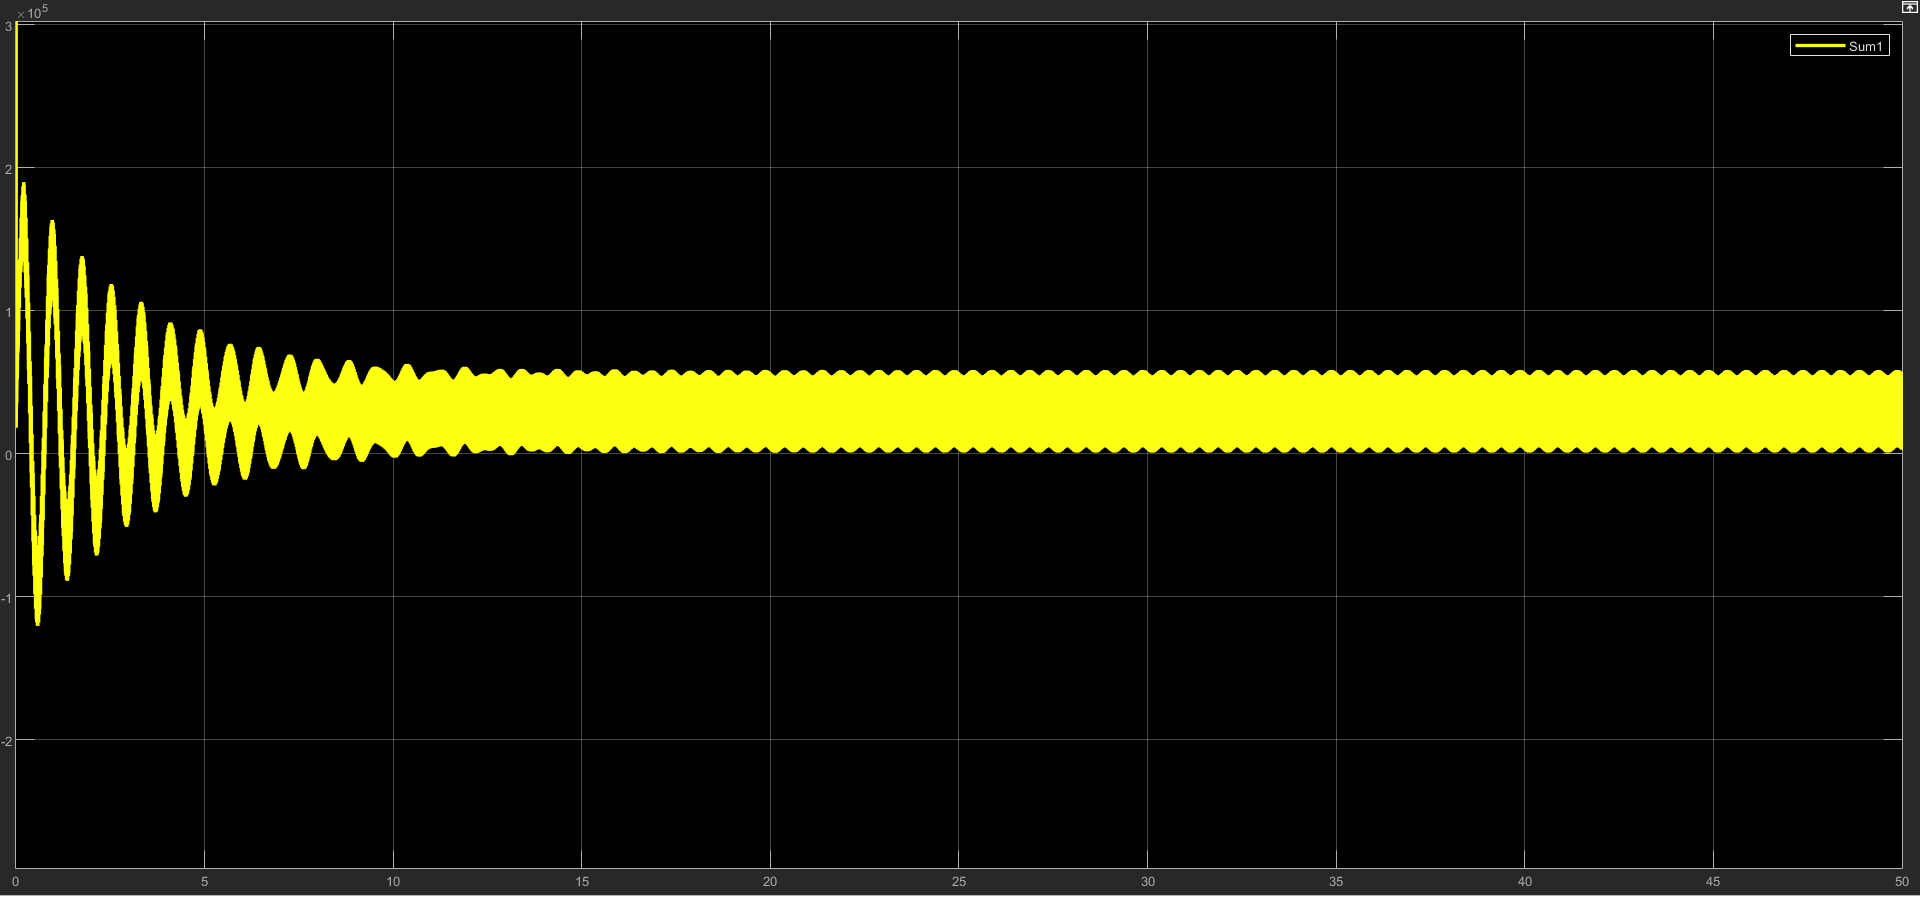
\includegraphics[scale = 0.4]{Q2_3_2_control2.png}
	\caption{سیگنال کنترلی با بزرگنمایی پس از اعمال اغتشاش بزرگتر با کنترلر 
		\lr{tube MPC}}
\end{figure}

همانطور که از تصاویر قابل مشاهده است،‌ اثر اغتشاش بسیار کاهش یافته است و سرعت سیستم نیز بالا رفته ولی سیگنال کنترلی نیز به شدت بزرگ شده است و برای خنثی سازی اغتشاش، حالت نوسانی پیدا کرده است. همچنین 
$x_4$
دچار فراجهش شده است که به خاطر بالا بودن ضرایب
\lr{PID}
است.

\newpage
\subsection{بخش چهارم}
در این قسمت به بررسی اثر نایقینی می‌پردازیم. برای این منظور، متغیرها به صورت زیر تغییر می‌کنند.
\begin{latin}
	\begin{lstlisting}[frame=single,numbers=left,style=Matlab-Pyglike]
function [xdot1, xdot2, xdot3, xdot4] = fcn(x1, x2, x3, x4, u, w, t)

% Parameter Values with uncertainity

m1 = 10000;
m1 = m1 + (m1/10) * sin(t);
m2 = 8000;
m2 = m2 + (m2/10) * sin(t);
k = 500000;
k = k + (k/20) * sin(t);
c = 5000;
c = c + (c/20) * sin(t);

% State-Equations

xdot1 = x3;
xdot2 = x4;
xdot3 = (1 / m1) * (k * (-x1 + x2) + c * (-x3 + x4) + u + w);
xdot4 = (1 / m2) * (k * (x1 - x2) + c * (x3 - x4));
	\end{lstlisting}
\end{latin}	

\newpage

سیگنال کنترلی و وضعیت سیستم با حالت بدون نایقینی تفاوت محسوسی ندارد.‌ ضرایب 
\lr{MPC}
همانند قبل است.
\begin{figure}[h!]
	\centering
	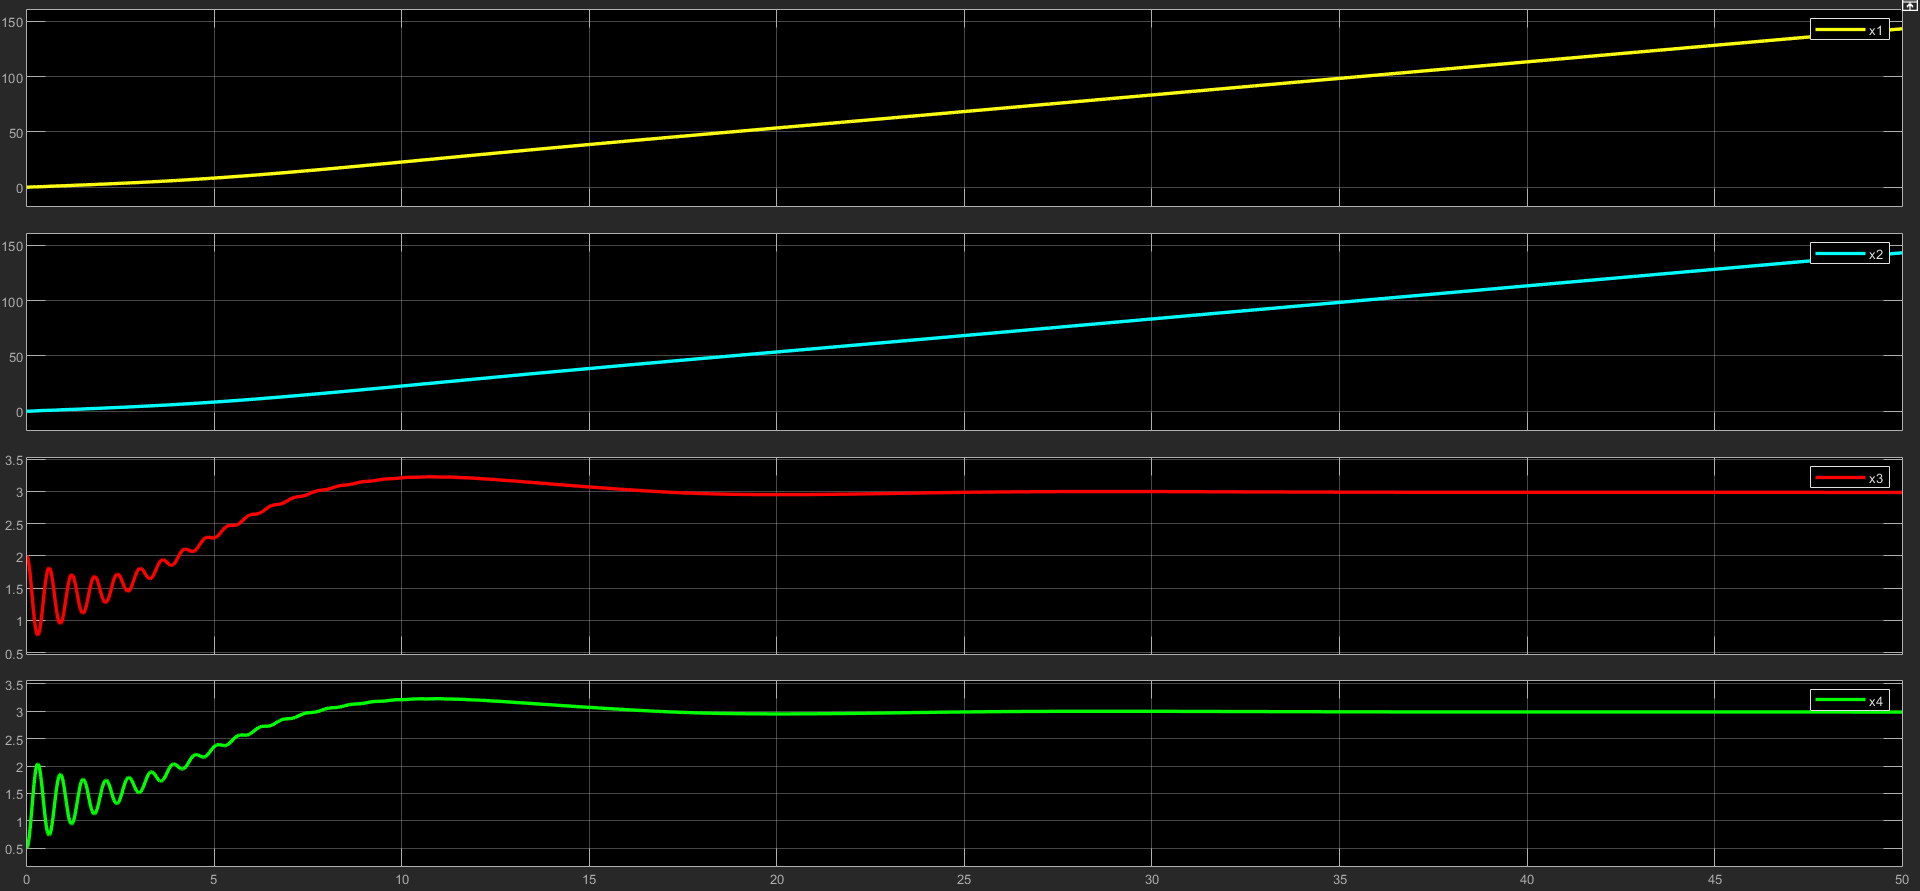
\includegraphics[scale = 0.4]{Q2_4_1_states.png}
	\caption{وضعیت 
		\lr{state}
		ها پس از اعمال نایقینی به سیستم با کنترلر 
		\lr{linear MPC}}
\end{figure}

\begin{figure}[h!]
	\centering
	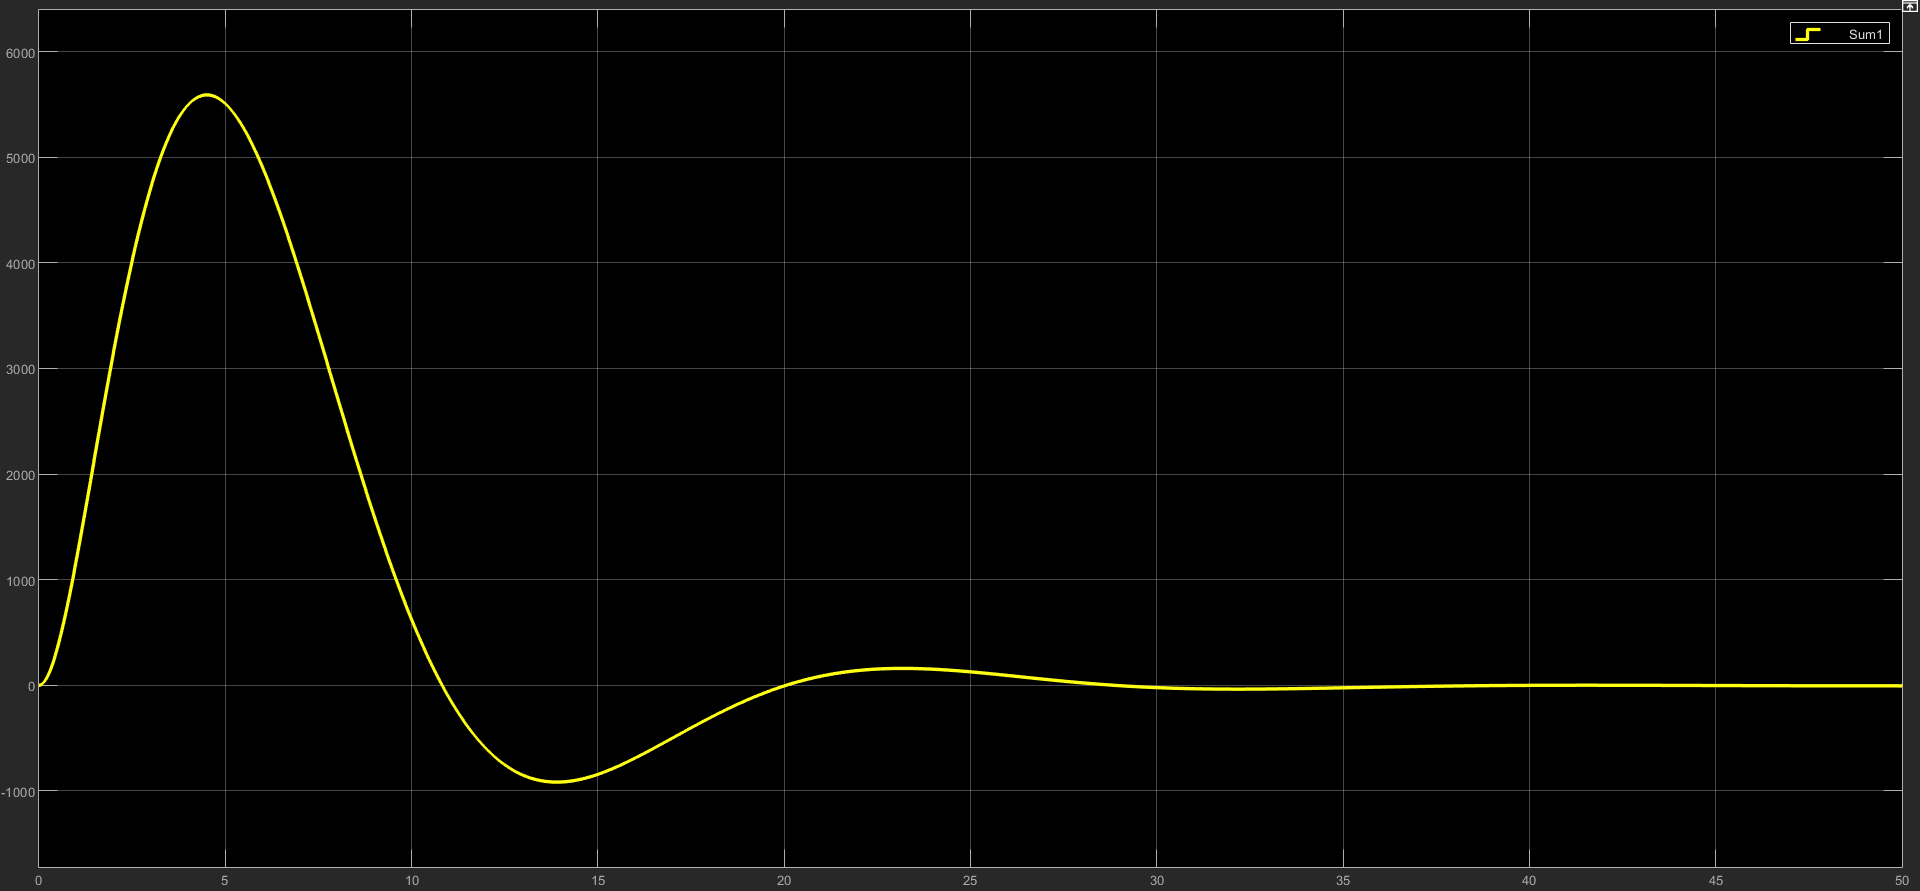
\includegraphics[scale = 0.4]{Q2_4_1_control.png}
	\caption{سیگنال کنترلی پس از اعمال نایقینی با کنترلر 
		\lr{linear MPC}}
\end{figure}

اگر از فاصله خیلی نزدیک وضعیت 
\lr{state}
ها را بررسی کنیم، مشاهده می‌کنیم که خطای ماندگاری در حال بزرگ شدن در سیستم است. مقدار این خطا در 50 ثانیه بسیار کوچک است.

\newpage
حال با کنترلر 
\lr{tube MPC}
خروجی‌های سیستم را بررسی می‌کنیم.
\begin{figure}[h!]
	\centering
	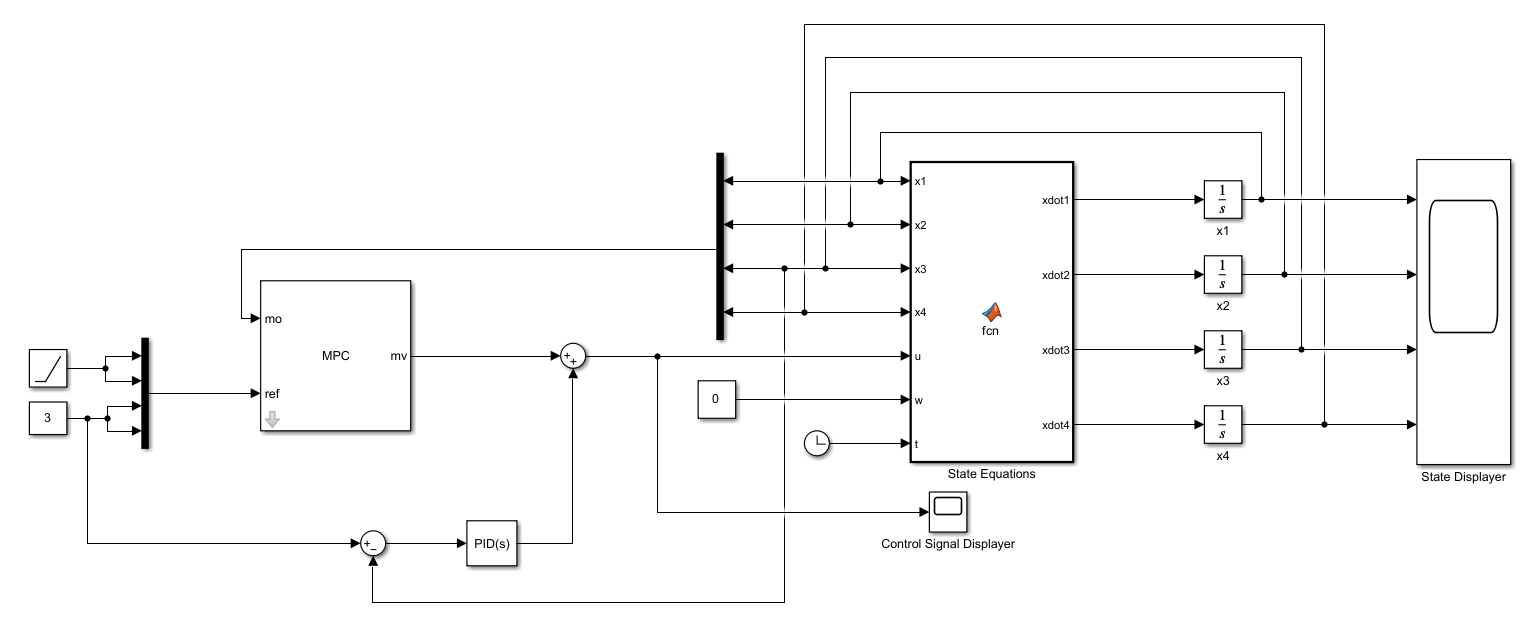
\includegraphics[scale = 0.5]{Q2_4_sim.png}
	\caption{سیستم دارای نایقینی با کنترلر 
		\lr{tube MPC}}
\end{figure}

\begin{figure}[h!]
	\centering
	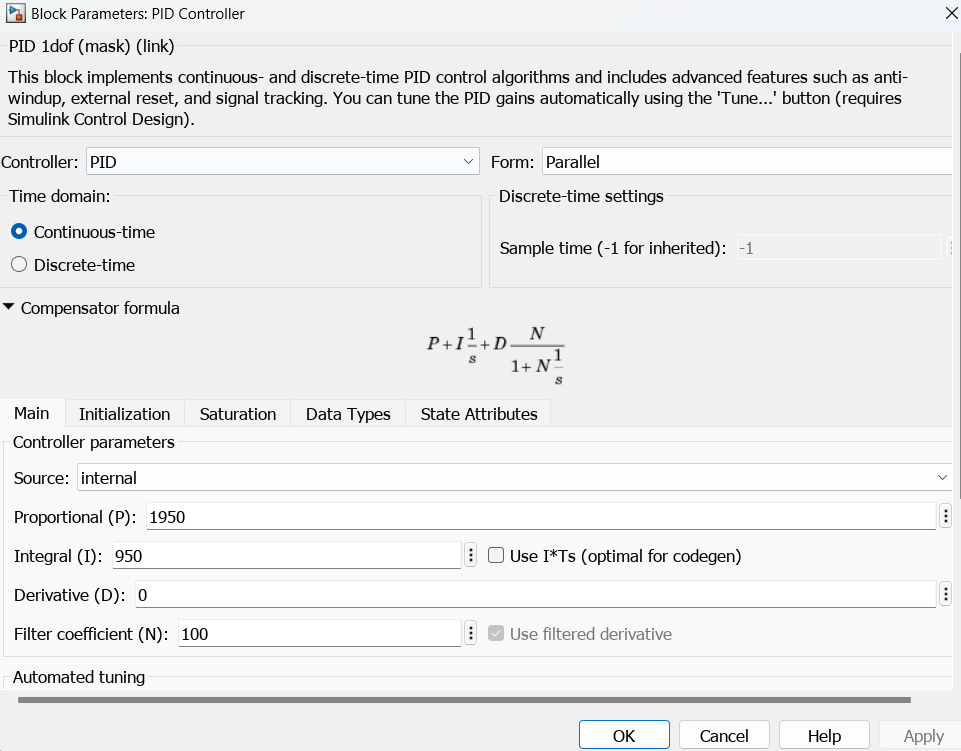
\includegraphics[scale = 0.5]{Q2_4_2_pid.png}
	\caption{ضرایب 
		\lr{PID}
		به کار رفته در 
		\lr{tub MPC}}
\end{figure}


\newpage
\begin{figure}[h!]
	\centering
	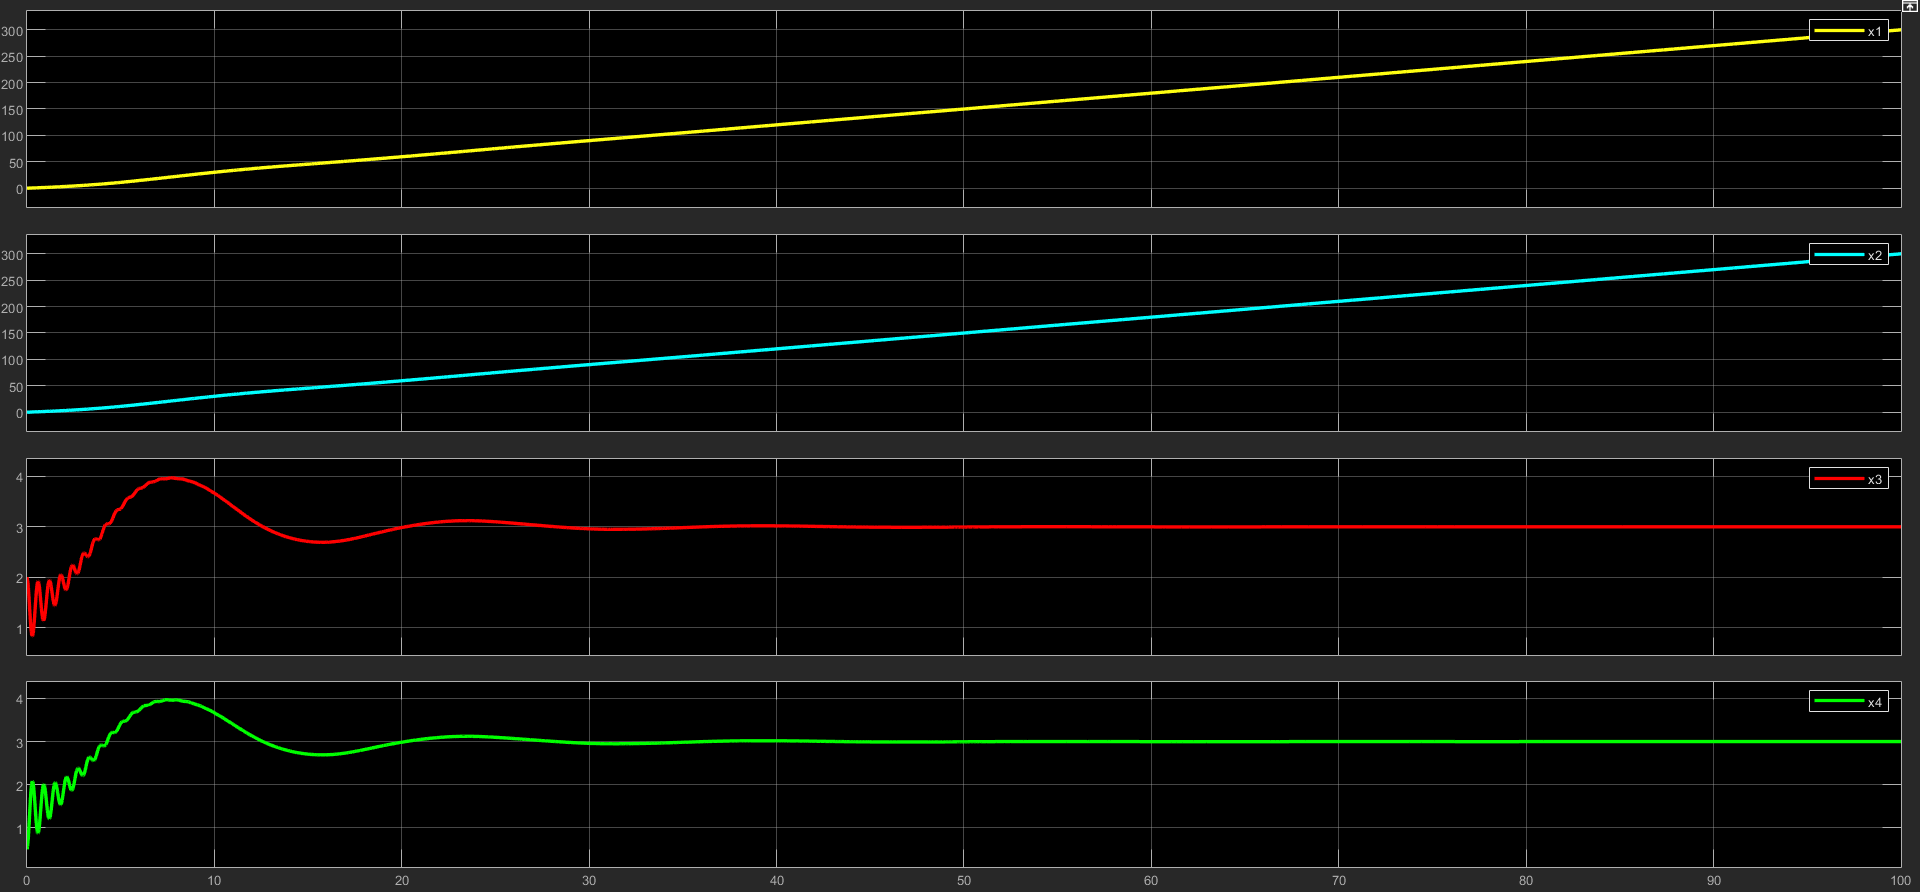
\includegraphics[scale = 0.4]{Q2_4_2_states.png}
	\caption{وضعیت 
		\lr{state}
		ها پس از اعمال نایقینی به سیستم با کنترلر 
		\lr{tube MPC}}
\end{figure}

با این کنترلر، خطای ماندگاری که در حال زیاد شدن بود از بین رفته و سیستم به سمت پایداری حرکت می‌کند.


\begin{figure}[h!]
	\centering
	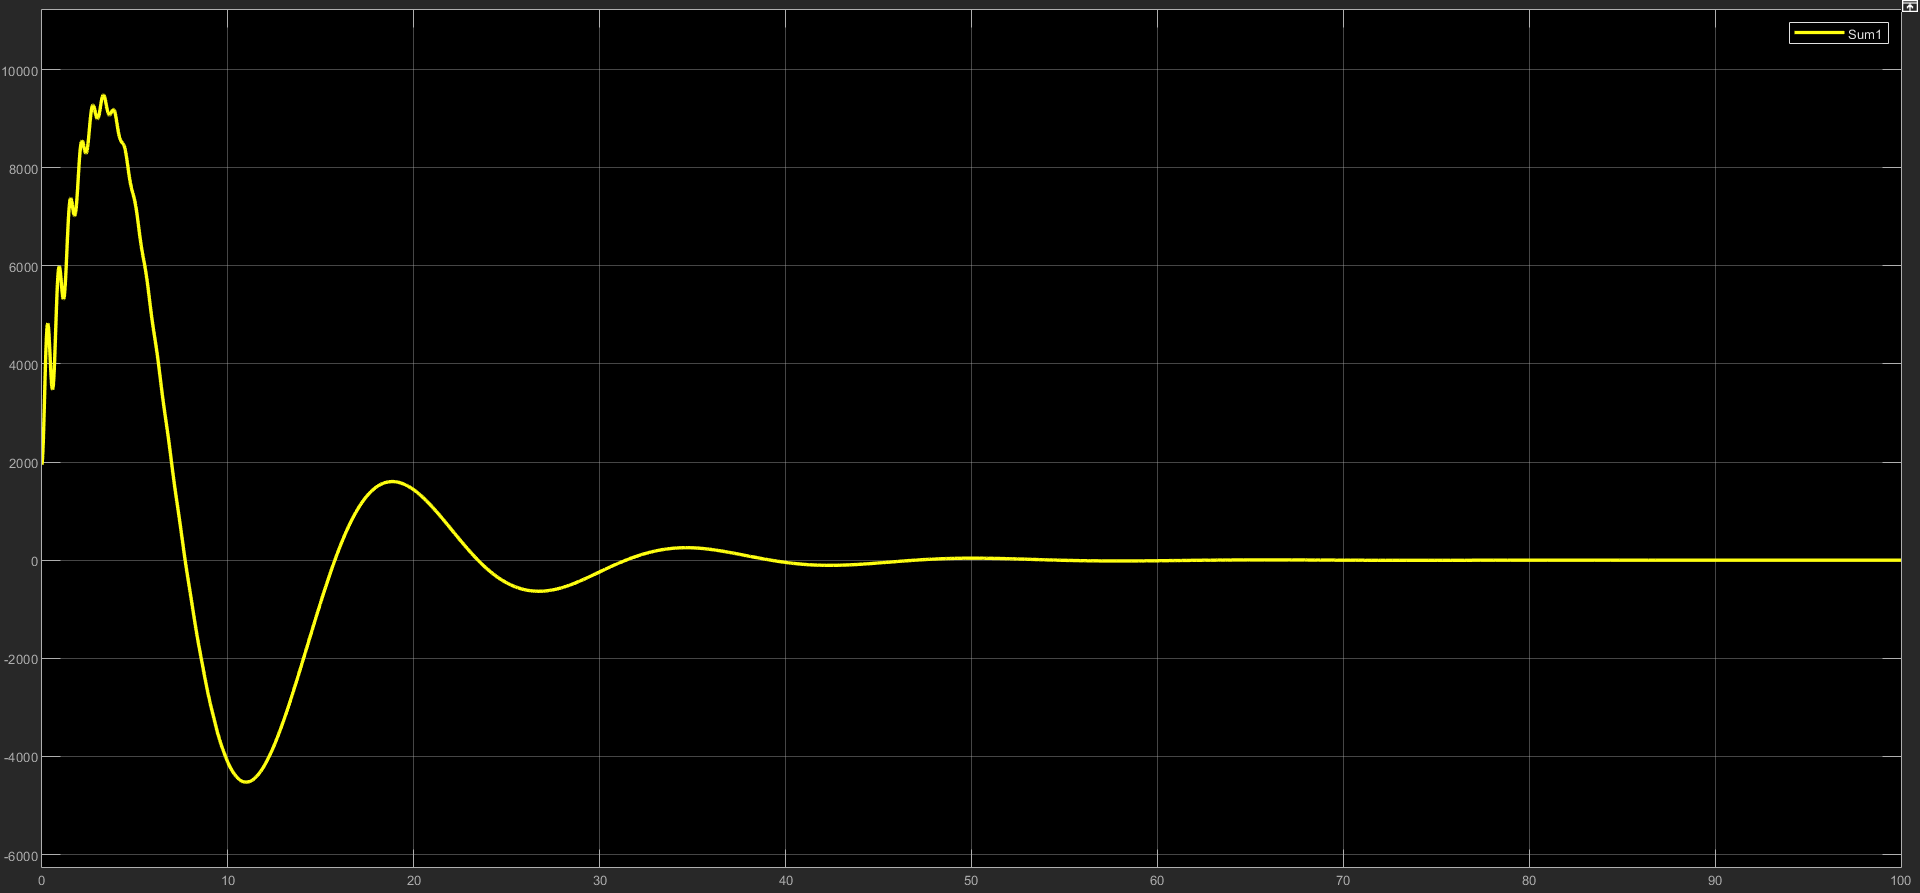
\includegraphics[scale = 0.4]{Q2_4_2_control.png}
	\caption{سیگنال کنترلی پس از اعمال نایقینی با کنترلر 
		\lr{tube MPC}}
\end{figure}

تفاوت سیگنال کنترلی با حالت قبل قابل مشاهده است.
\end{document} 
